\documentclass[a4paper, 12pt]{extarticle}

\usepackage{arxiv}

\usepackage[T2A]{fontenc}
\usepackage[utf8]{inputenc}
\usepackage[english, russian]{babel}
% \usepackage{cmap}
\usepackage{url}
\usepackage{booktabs}
\usepackage{nicefrac}
\usepackage{microtype}
\usepackage{lipsum}
\usepackage{graphicx}
\usepackage{epstopdf}
\usepackage{subfig}
\usepackage[square,sort,comma,numbers]{natbib}
\usepackage{doi}
\usepackage{multicol}
\usepackage{multirow}
\usepackage{tabularx}
\usepackage{float}

\usepackage{tikz}
\usetikzlibrary{matrix}

% Algorithms
\usepackage{algpseudocode}
\usepackage{algorithm}

%% Шрифты
\usepackage{euscript} % Шрифт Евклид
\usepackage{mathrsfs} % Красивый матшрифт
\usepackage{extsizes} % Возможность сделать 14-й шрифт
\usepackage{bm}

\usepackage{makecell} % diaghead in a table
\usepackage{amsmath,amsfonts,amssymb,amsthm,mathtools,dsfont}
\usepackage{icomma}
\usepackage[labelfont=bf]{caption}
\usepackage{subfig} % for subfigures
\usepackage{wrapfig}

\newcommand{\bz}{\mathbf{z}}
\newcommand{\bx}{\mathbf{x}}
\newcommand{\by}{\mathbf{y}}
\newcommand{\bv}{\mathbf{v}}
\newcommand{\bw}{\mathbf{w}}
\newcommand{\ba}{\mathbf{a}}
\newcommand{\bb}{\mathbf{b}}
\newcommand{\bp}{\mathbf{p}}
\newcommand{\bq}{\mathbf{q}}
\newcommand{\bt}{\mathbf{t}}
\newcommand{\bu}{\mathbf{u}}
\newcommand{\bs}{\mathbf{s}}
\newcommand{\bT}{\mathbf{T}}
\newcommand{\bX}{\mathbf{X}}
\newcommand{\bZ}{\mathbf{Z}}
\newcommand{\bS}{\mathbf{S}}
\newcommand{\bH}{\mathbf{H}}
\newcommand{\bW}{\mathbf{W}}
\newcommand{\bY}{\mathbf{Y}}
\newcommand{\bU}{\mathbf{U}}
\newcommand{\bQ}{\mathbf{Q}}
\newcommand{\bP}{\mathbf{P}}
\newcommand{\bA}{\mathbf{A}}
\newcommand{\bB}{\mathbf{B}}
\newcommand{\bC}{\mathbf{C}}
\newcommand{\bE}{\mathbf{E}}
\newcommand{\bF}{\mathbf{F}}
\newcommand{\bomega}{\boldsymbol{\omega}}
\newcommand{\btheta}{\boldsymbol{\theta}}
\newcommand{\bgamma}{\boldsymbol{\gamma}}
\newcommand{\bdelta}{\boldsymbol{\delta}}
\newcommand{\bPsi}{\boldsymbol{\Psi}}
\newcommand{\bpsi}{\boldsymbol{\psi}}
\newcommand{\bxi}{\boldsymbol{\xi}}
\newcommand{\bchi}{\boldsymbol{\chi}}
\newcommand{\bzeta}{\boldsymbol{\zeta}}
\newcommand{\blambda}{\boldsymbol{\lambda}}
\newcommand{\beps}{\boldsymbol{\varepsilon}}
\newcommand{\bZeta}{\boldsymbol{Z}}
% mathcal
\newcommand{\cX}{\mathcal{X}}
\newcommand{\cY}{\mathcal{Y}}
\newcommand{\cW}{\mathcal{W}}

\newcommand{\dH}{\mathds{H}}
\newcommand{\dR}{\mathds{R}}
% transpose
\newcommand{\T}{^{\mathsf{T}}}

% \renewcommand{\shorttitle}{\textit{arXiv} Шаблон}
\renewcommand{\epsilon}{\ensuremath{\varepsilon}}
\renewcommand{\phi}{\ensuremath{\varphi}}
\renewcommand{\kappa}{\ensuremath{\varkappa}}
\renewcommand{\le}{\ensuremath{\leqslant}}
\renewcommand{\leq}{\ensuremath{\leqslant}}
\renewcommand{\ge}{\ensuremath{\geqslant}}
\renewcommand{\geq}{\ensuremath{\geqslant}}
\renewcommand{\emptyset}{\varnothing}

\DeclareMathOperator*{\argmax}{arg\,max}  % in your preamble
\DeclareMathOperator*{\argmin}{arg\,min}  % in your preamble 

\usepackage{hyperref}
% \usepackage[usenames,dvipsnames,svgnames,table,rgb]{xcolor}

\hypersetup{
	unicode=true,
	colorlinks=true,
	linkcolor=black,        % внутренние ссылки
	citecolor=blue,         % на библиографию
	filecolor=magenta,      % на файлы
	urlcolor=blue           % на URL
}

\graphicspath{{./figures}}

\usepackage{enumitem} % Для модификаций перечневых окружений

\theoremstyle{definition} % "Определение"
\newtheorem{definition}{Опр.}[section]

\usepackage{etoolbox}

\makeatletter
\expandafter\patchcmd\csname\string\algorithmic\endcsname{\itemsep\z@}{\itemsep=1.5mm}{}{}
\makeatother

\newcommand{\myfigref}[2]{~\ref{#1}.\subref{#2}}% <---- a new macro for referring to a subfigure
\renewcommand{\abstractname}{Аннотация}

\title{Восстановление снимков фМРТ по просматриваемому видеоряду}

\author{
	Дорин Даниил \\
	\texttt{dorin.dd@phystech.edu} \\
	\And
	Киселев Никита \\
	\texttt{kiselev.ns@phystech.edu} \\
	\And
	Грабовой Андрей \\
	\texttt{grabovoy.av@phystech.edu}
}
\date{\today}

\begin{document}
\maketitle

\begin{abstract}

	Исследуется проблема восстановления зависимости между показаниями датчиков фМРТ
	и восприятием внешнего мира человеком.
	Проводится анализ зависимости между последовательностью снимков фМРТ и видеорядом,
	просматриваемым человеком.
	На основе исследования зависимости предлагается метод аппроксимации показаний фМРТ по
	просматриваемому видеоряду. Метод строится в предположении наличия неизменяющегося
	времени гемодинамической ответной реакции зависимости уровня кислорода в крови. 
	Для каждого вокселя снимка фМРТ независимо строится линейная модель. 
	Используется предположение марковости последовательности снимков фМРТ.
	Для анализа предложенного метода проводится вычислительный эксперимент на
	выборке, полученной при томографическом обследовании большого числа испытуемых.
	На экспериментальных данных проводится анализ зависимости 
	качества работы метода от времени гемодинамической ответной реакции.
	Проверяются гипотезы об инвариантности весов модели относительно человека
	и корректности построенного метода.

\end{abstract}


\keywords{нейровизуализация \and фМРТ \and видеоряд \and зависимость между данными
\and проверка гипотез \and линейная модель}

\section{Введение}

Совокупность методов, визуализирующих структуру и функции человеческого мозга,
называется \textit{нейровизуализацией}. Методы нейровизуализации \citep{puras2014neurovisualization}, такие как ЭКГ, КТ, МРТ и фМРТ,
используются для изучения мозга, а также для обнаружения заболеваний и психических расстройств.

\textit{Функциональная магнитно-резонансная томография} или \textit{фМРТ} (англ.~\textit{fMRI})
является разновидностью магнитно-резонансной томографии и основана на изменениях в токе крови,
вызванных нейронной активностью мозга \citep{Glover2011}.
Эти изменения происходят не моментально, а с некоторой задержкой,
которая составляет 4--8 с \citep{Bandettini1992}.
Она возникает из-за того, что сосудистая система достаточно долго реагирует
на потребность мозга в глюкозе \citep{Ogawa1990, LEBIHAN1995231, Logothetis2003}. 

При получении снимков фМРТ используются последовательности
эхопланарных изображений (EPI) \citep{Connelly1993, Kwong1992, Ogawa1992}.
Обработка участков с изменяющейся интенсивностью сигнала в
зависимости от способа активации, вида артефактов и длительности
проводится с помощью специальных методов и программ 
\citep{Bandettini1992, BAUDENDISTEL1995701, COX1996162}.
Обработанные результаты оформляются в виде карт активации,
которые совмещаются с локализацией анатомических образований
головконого мозга.

Метод фМРТ играет большую роль в нейровизуализации, однако имеет ряд важных ограничений.
В работах \citep{menon1999spatial, logothetis2008we} рассматриваются
временное и пространственное разрешения фМРТ. Временное разрешение является существенным
недостатком данного метода. Другой недостаток фМРТ~--- неизбежно возникающие шумы,
связанные с движением объекта в сканере, сердцебиением и дыханием человека, тепловыми
флуктуациями самого прибора и т.\,д. В работе \citep{1804.10167} предлагаются методы
подавления вышеперечисленных шумов на основе графов и демонстрируется их эффективность в задаче
выявления эпилепсии и депрессии.

При проведении фМРТ испытуемому дают различные тест-задания и
применяют внешние раздражители, вызывающие активацию определенных
локальных участков головного мозга, ответственных за выполнение
соответствующих его функций.
Применяются различные тест-задания: движения пальцами и конечностями
\citep{Roux1998, Papke1999}, поиск изображения и рассмотрение
шахматной доски \citep{Engel1994, Schneider1994},
прослушивание неспецифичных шумов, единичных слов
или связного текста \citep{Binder1994, Dymarkowski1998}.
Причиной изменения активности человеского мозга во время фМРТ-обследования
также может служить просмотр видеоматериала \citep{decety1997brain},
что является предметом исследования настоящей работы. 

Наиболее известные методы обработки видео основаны на 3D свертках \citep{tran2015learning}.
Отличие 3D от 2D сверток заключается в одновременной работе с пространственной и временной частью
информации. Существенный недостаток данных методов — сильное увеличение числа параметров модели и
большие вычислительные затраты. Одной из наиболее современных и улучшаемых архитектур
нейронных сетей для обработки изображений является остаточная нейронная сеть ResNet~\citep{he2015deep}.
Она позволяет обучать глубокие нейронные сети (до 152 слоев) с высокой точностью,
преодолевая проблему затухания градиента, которая возникает при обучении глубоких сетей.

Настоящая работа посвящена восстановлению зависимости между снимками фМРТ и видеорядом.
Используется предположение, что такая зависимость существует.
Кроме того, предполагается, что между снимком и видеорядом есть постоянная задержка во времени
\citep{Logothetis2003}.
Проверяется зависимость снимка фМРТ от одного изображения и предыдущего снимка.
Время задержки выступает в качестве гиперпараметра модели.
На основе анализа зависимости предлагается метод аппроксимации показаний фМРТ по
просматриваемому видеоряду.

Согласно исследованию \citep{anderson2006}, при фМРТ-обследовании пациентов,
просматривающих видеоряд, активируется определенная корковая сеть. Она включает
в себя в том числе задние центральные и фронтальные области. Находится эта сеть
преимущественно в правом полушарии. В настоящей работе рассматривается подход,
использующий для анализа времени задержки именно эти части головного мозга.

Данные, на которых проводятся проверка гипотезы зависимости и демонстрация работы построенного
метода, представлены в работе \citep{Berezutskaya2022}. Этот набор данных был получен при
обследовании группы из 63 испытуемых. Тридцать из них проходили обследование фМРТ.
Им предлагалось выполнить одно и то же задание~--- просмотреть короткий аудиовизуальный фильм.
Для него в рассматриваемой работе были сгенерированы аннотации, содержащие в том числе информацию о времени появления и исчезновения
отдельных слов, объектов и персонажей. Методы аудио- и видеоаннотирования подробно излагаются в
\citep{boersma2018praat} и \citep{Berezutskaya2020}.

\section{Постановка задачи}

Задана частота кадров $\nu \in \mathbb{R}$ и продолжительность $t \in \mathbb{R}$ видеоряда.
Задан видеоряд
\begin{equation}
	\label{eq1}
	\bP = [\bp_1, \ldots, \bp_{\nu t}], \quad\
	\bp_{\ell} \in \mathbb{R}^{W \times H \times C},
\end{equation}
с шириной, высотой и числом каналов изображения $W, H$ и
$C$ соответственно.

Обозначим частоту снимков фМРТ $\mu \in \mathbb{R}$. Задана последовательность снимков
\begin{equation}
	\label{eq2}
	\bS = [\bs_1, \ldots, \bs_{\mu t}], \quad\
	\bs_{\ell} \in \mathbb{R}^{X \times Y \times Z},
\end{equation}
где $X, Y$ и $Z$~--- размерности воксельного изображения.

Задача состоит в построении отображения, которое бы учитывало задержку $\Delta t$ между
снимком фМРТ и видеорядом, а также предыдущие томографические показания. Формально, необходимо
найти такое отображение $\mathbf{g}$, что
\begin{equation}
	\label{eq3}
	\mathbf{g}(\bp_1, \ldots, \bp_{k_{\ell} - \nu \Delta t}; \bs_1, \ldots, \bs_{\ell-1}) = \bs_{\ell},
	\ \ell = 1, \ldots, \mu t,
\end{equation}
где для $\ell$-го снимка фМРТ номер соответствующего изображения $k_{\ell}$ определяется по формуле
\begin{equation}
	\label{eq4}
	k_{\ell} = \dfrac{\ell \cdot \nu}{\mu}.
\end{equation}

\section{Предлагаемый метод восстановления снимков фМРТ}

Схема предлагаемого метода восстановления снимков фМРТ приведена на Рис.~\ref{fig:scheme}.

\begin{figure}[h!]
	\centering
	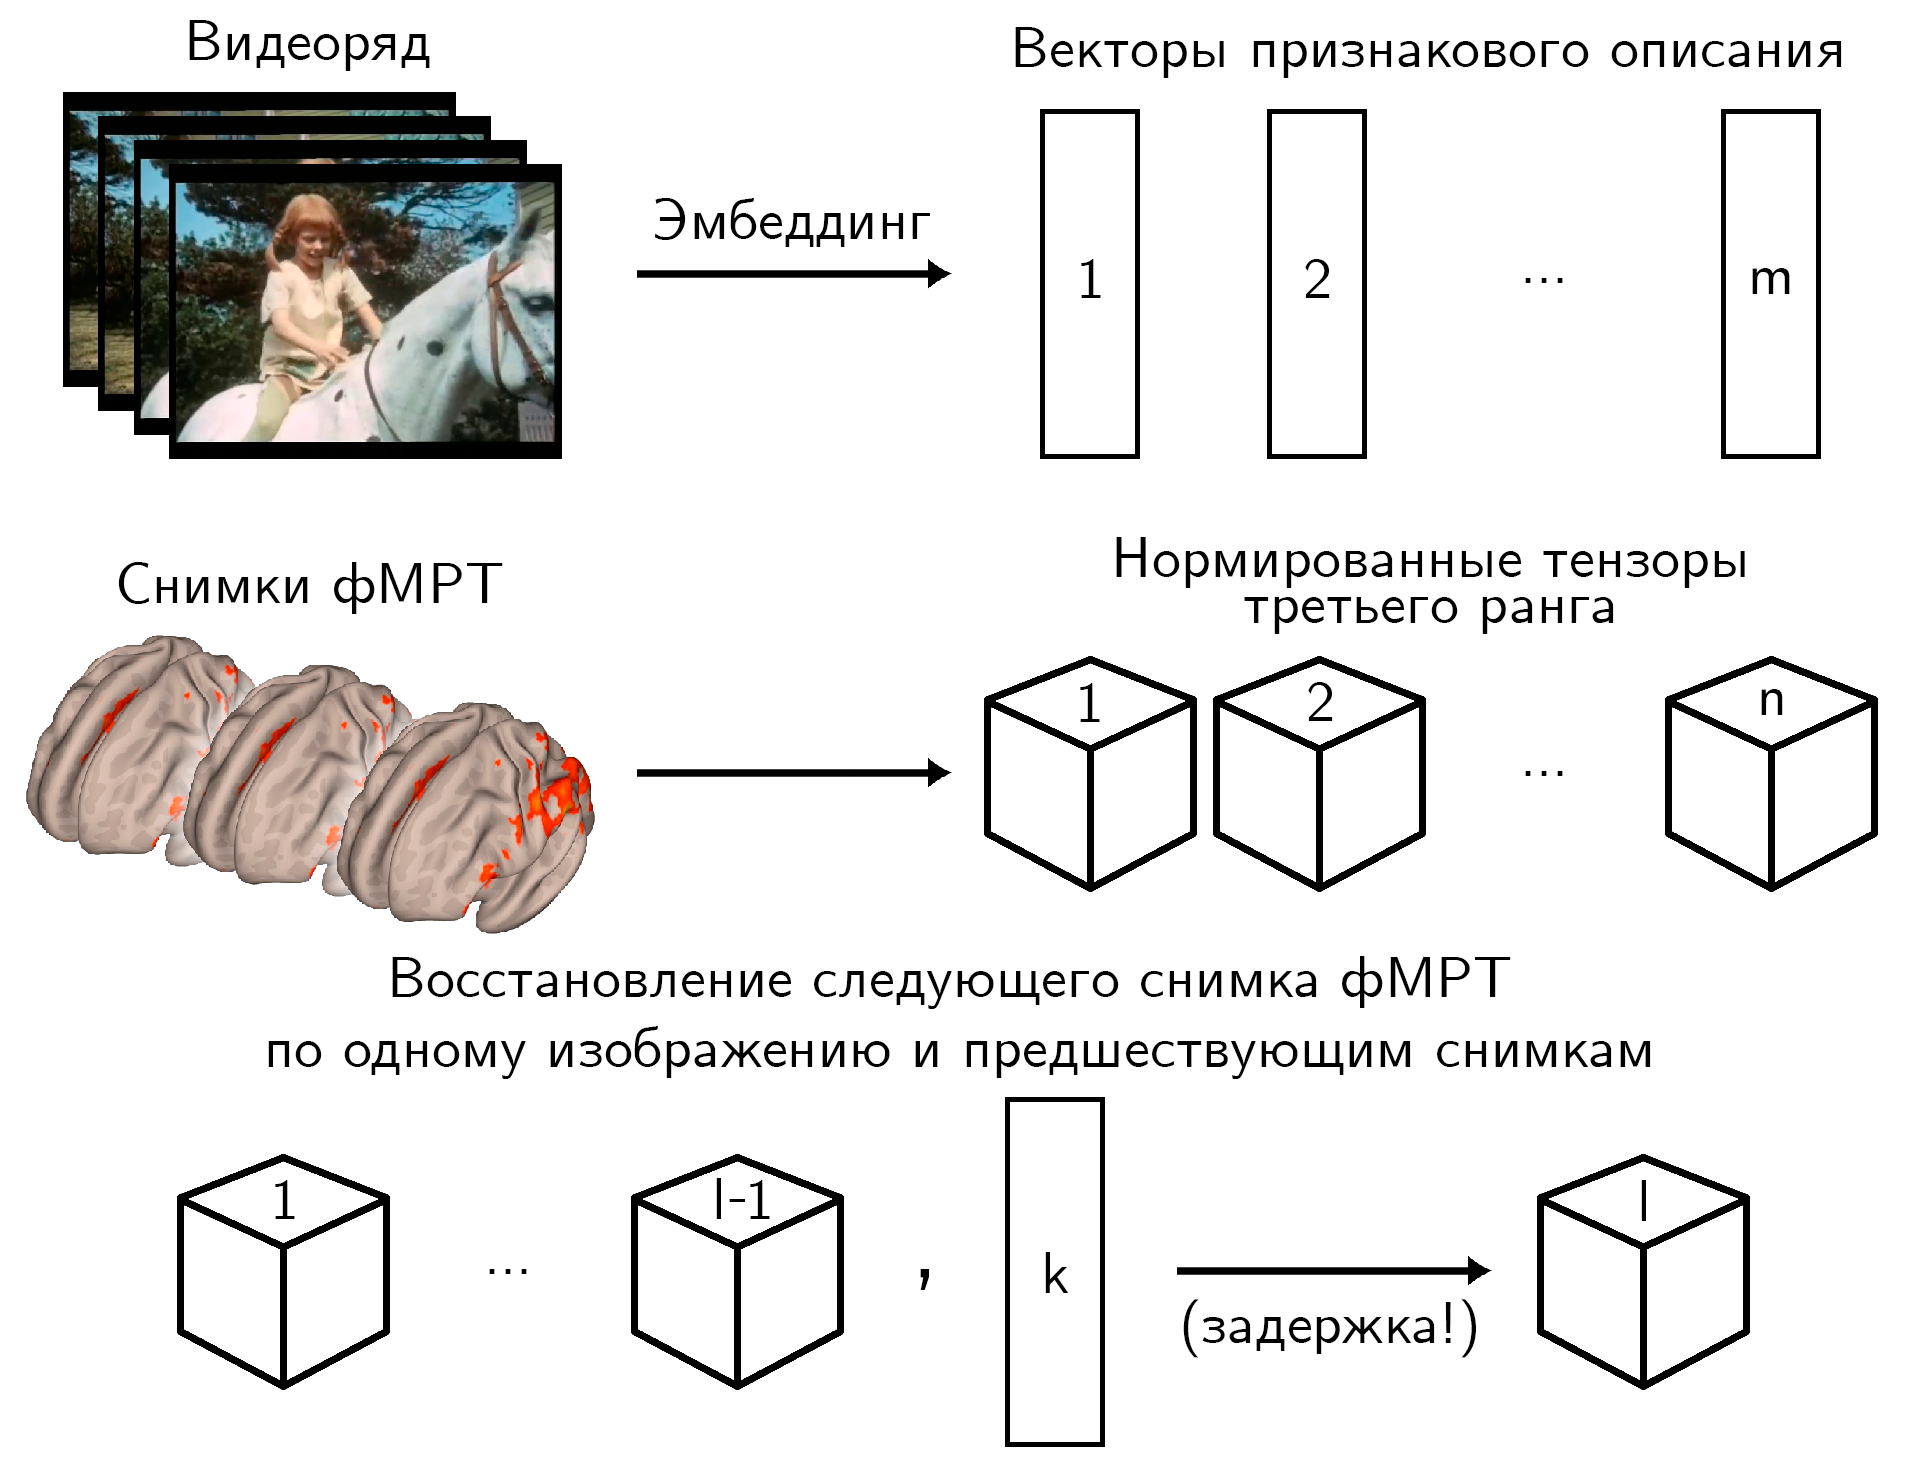
\includegraphics[width=0.8\textwidth]{scheme.png}
	\caption{Схема метода}
	\label{fig:scheme}
\end{figure}

Обозначим снимок фМРТ как $\bs_{\ell} = [v^{\ell}_{ijk}] \in \mathbb{R}^{X \times Y \times Z}$,
где $v^{\ell}_{ijk} \in \mathbb{R}_+$~--- значение соответствующего вокселя.
С целью сокращения времени работы метода предлагается использовать сжатие снимков фМРТ путем уменьшения размерностей.
Сжатие в 2 раза представляется в виде отображения
\[\bm{\chi}: \mathbb{R}^{X \times Y \times Z} \to \mathbb{R}^{X/2 \times Y/2 \times Z/2}.\]
Сжатие в $2^k$ раз получается применением $\bm{\chi}$ последовательно $k$ раз. 
Далее для простоты сохраняем обозначения размерностей снимков $X \times Y \times Z$.

Предположим, что для последовательности снимков выполнено марковское свойство,
т.е. каждый снимок зависит только от одного изображения и предыдущего снимка.
Тогда соответствующее отображение записывается в виде
\begin{equation}
	\label{eq5}
	\mathbf{g}(\bp_{k_{\ell} - \nu \Delta t}) = \bs_{\ell} - \bs_{\ell-1} = \bdelta_{\ell}, \ \ell = 2, \ldots, \mu t.
\end{equation}
где $\bdelta_{\ell} = [v^{\ell}_{ijk} - v^{\ell-1}_{ijk}] = [\delta^{\ell}_{ijk}] \in \mathbb{R}^{X \times Y \times Z}$~--- разность между двумя последовательными снимками.

Отображение $\mathbf{g}: \mathbf{P} \to \mathbf{S}$ представляется в виде композиции
двух других:
\[ \mathbf{g} = \bm{\varphi} \circ \bm{\psi}, \]
\vspace{-0.8cm}
\begin{align*}
	 & \bm{\psi}: \mathbf{P} \to \mathbb{R}^d
	\text{~--- векторизация изображения,}        \\
	 & \bm{\varphi}: \mathbb{R}^d \to \mathbf{S}
	\text{~--- восстанавливаемое отображение.}
\end{align*}

Для каждого изображения из видеоряда имеем вектор признакового описания размерности $d$:
\[ \bx_{\ell} = [x^{\ell}_1, \ldots, x^{\ell}_{d}]\T \in \mathbb{R}^{d}, \ {\ell} = 1, \ldots, \nu t. \]
Используется архитектура нейронной сети ResNet152 без последнего линейного слоя.

Учитывая \eqref{eq4}, суммарное число пар (изображение, снимок)
равно $N = \mu (t - \Delta t)$. Таким образом, для каждого вокселя задана выборка
\[ \mathfrak{D}_{ijk} = \{(\bx_{\ell}, \delta^{\ell}_{ijk}) \ | \ {\ell} = 2, \ldots, N \}. \]

Поставлена задача восстановления регрессии
\begin{equation}
	\label{eq6}
	y_{ijk}: \mathbb{R}^{d} \to \mathbb{R}.
\end{equation}

Используется линейная модель с вектором параметров
\[ \bw_{ijk} = [w^{ijk}_1, \ldots, w^{ijk}_{d}]\T \in \mathbb{R}^{d}: \]
\begin{equation}
	\label{eq7}
	f_{ijk}(\bx, \bw_{ijk}) = \langle \bx, \bw_{ijk} \rangle.
\end{equation}

Для модели $f_{ijk}$ с соответствующим ей вектором параметров $\bw_{ijk} \in \mathbb{R}^{d}$
определим квадратичную функцию потерь с $L_2$ регуляризацией:
\begin{equation}
	\label{eq8}
	\mathcal{L}_{ijk}(\bw_{ijk}) = \sum\limits_{\ell = 2}^{N} \big(f_{ijk}(\bx_{\ell}, \bw_{ijk}) - \delta^{\ell}_{ijk}\big)^2 + \alpha \| \bw_{ijk} \|_2^2,
\end{equation}
где $\alpha \in \mathbb{R}$~--- коэффициент регуляризации.

Требуется найти параметры, доставляющие минимум функционалу потерь $\mathcal{L}_{ijk}(\bw_{ijk})$
при заданных гиперпараметрах $\Delta t$ и $\alpha$:
\begin{equation}
	\label{eq9}
	\hat{\bw}_{ijk} = \argmin_{\bw_{ijk}} \mathcal{L}_{ijk}(\bw_{ijk}).
\end{equation}

Минимум функции потерь находится методом наименьших квадратов. Определим матрицу объектов-признаков
\begin{equation}
	\label{eq10}
	\bX = [\bx_2, \ldots, \bx_N]\T = [x^i_j] \in \mathbb{R}^{(N-1) \times d}
\end{equation}
и вектор, компонентами которого являются разности значений одного и того же вокселя в разных снимках,
\begin{equation}
	\label{eq11}
	\mathbf{\Delta}_{ijk} = [\delta^2_{ijk}, \ldots, \delta^N_{ijk}]\T \in \mathbb{R}^{N-1}.
\end{equation}

Решение записывается в виде
\begin{equation}
	\label{eq12}
	\hat{\bw}_{ijk} = (\bX\T \bX + \alpha \mathbf{I})^{-1} \bX\T \mathbf{\Delta}_{ijk}.
\end{equation}

Получим формулу для восстановленных снимков фМРТ. Введем матрицу весов
\begin{equation}
	\label{eq13}
	\hat{\bW} = [\hat{\bw}_1, \ldots, \hat{\bw}_{XYZ}]\T = [\hat{w}^i_j] \in \mathbb{R}^{XYZ \times d}.
\end{equation}

Введем для тензоров $\bs_{\ell}, \bdelta_{\ell} \in \mathbb{R}^{X \times Y \times Z}$ векторы
\[ \bs_{\ell}^{R} = [ v^{\ell}_1, \ldots, v^{\ell}_{XYZ} ]\T,\
	\bdelta_{\ell}^{R} = [ \delta^{\ell}_1, \ldots, \delta^{\ell}_{XYZ} ]\T \in \mathbb{R}^{XYZ}. \]

Тогда вектор восстановленного снимка находится по формуле
\begin{equation}
	\label{eq14}
	\hat{\bs}_{\ell}^{R} = \bs_{\ell-1}^{R} + \hat{\bdelta}_{\ell}^{R} = \bs_{\ell-1}^{R} + \hat{\mathbf{W}} \mathbf{x}_{\ell}.
\end{equation}

\section{Вычислительный эксперимент}

Для анализа работоспособности предложенного метода и проверки гипотез
проведен вычислительный эксперимент.

В качестве данных использовалась выборка, представленная в работе \citep{Berezutskaya2022}.
Набор данных содержит результаты обследования 63 испытуемых.
Для тридцати из них известны показания фМРТ.
Среди них 16 мужчин и 14 женщин в возрасте от 7 до 47 лет.
Средний возраст испытуемого~--- 22 года.

Характеристики выборки: продолжительность обследования,
частота кадров видеоряда и снимков фМРТ, размерности изображений
и снимков приведены в Таблице~\ref{table:sample}.

\begin{table}[h!]
	\centering
	\caption{Описание выборки}
	\begin{tabular}{|c|c|c|}
		\hline
		Название                       & Обозначение & Значение             \\
		\hline \hline
		Продолжительность обследования & $t$         & 390 с                \\ \hline
		Частота кадров видео           & $\nu$       & 25 $\text{с}^{-1}$   \\ \hline
		Частота снимков фМРТ           & $\mu$       & 1.64 $\text{с}^{-1}$ \\ \hline
		Размерности изображения        & $W, H, C$   & 640, 480, 3          \\ \hline
		Размерности снимка             & $X, Y, Z$   & 40, 64, 64           \\ \hline
	\end{tabular}
	\label{table:sample}
\end{table}

Произведено разделение выборки на тренировочную и тестовую в соотношении 70\% и 30\% соответственно.
Критерием качества восстановления снимка фМРТ служит MSE~--- сумма квадратов отклонений
между истинным и восстановленным снимками, усредненная по всем вокселям каждого снимка
из тестовой выборки.

Для сокращения времени работы алгоритма производится предварительное сжатие снимка фМРТ
с помощью слоя MaxPool3D. Рассматриваются коэффициенты сжатия 1, 2, 4 и 8.
Значения вокселей нормализуются на $[0; 1]$ процедурой MinMaxScale.

В Таблице~\ref{table:pc} приведены технические характеристики компьютера, на котором
производился вычислительный эксперимент.

\begin{table}[h!]
	\centering
	\caption{Технические характеристики компьютера}
	\begin{tabular}{|c|c|}
		\hline
		Элемент & Описание \\
		\hline \hline
		Процессор & Intel Core i7-7700 3.6 GHz \\ \hline
		Оперативная память & 16 GB 2400 MHz \\ \hline
		Видеокарта & NVIDIA GeForce GTX 1060 3 GB \\ \hline
		Жесткий диск & M.2 SSD \\ \hline
		Операционная система & Windows 10 \\ \hline
	\end{tabular}
	\label{table:pc}
\end{table}

\paragraph*{Демонстрация работы метода.}

На Рис.~\ref*{fig:example} представлены срезы истинного и восстановленного снимков из
тестовой выборки. На Рис.\myfigref{fig:example}{fig:example-c} изображена разность между ними.
Для демонстрации работы алгоритма был выбран 7-ой испытуемый, $\Delta t = 5 \text{ с}$, коэффициент сжатия 1, коэффициент регуляризации
$\alpha = 1000$. Рассмотрен 20-ый срез по первой координате 37-го снимка в последовательности.
Так как значения вокселей нормированы на отрезок $[0; 1]$, то ошибка порядка $10^{-3}$
свидетельствует о достаточно точном предсказании.

\begin{figure}[h!]
	\centering
	\subfloat[Истинный]{\label{fig:example-a}{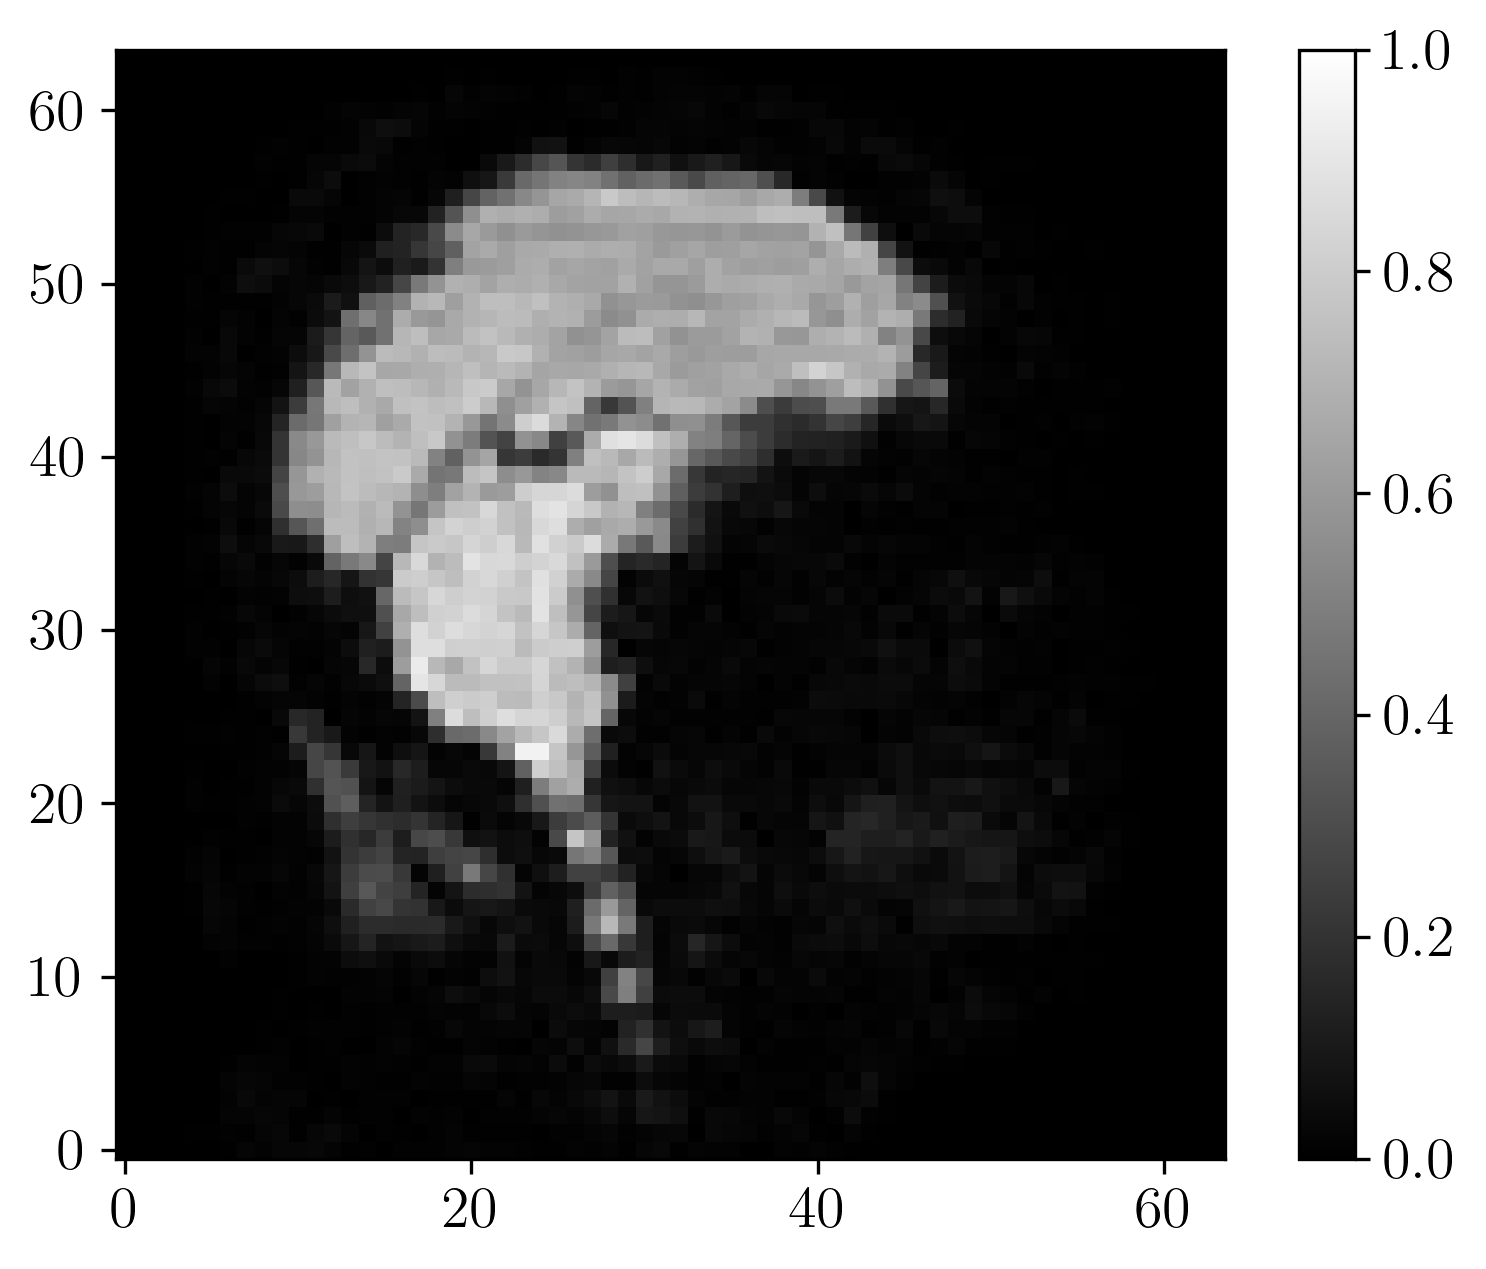
\includegraphics[width=0.33\textwidth]{sub-07-5-1-1000-37-20-_-_-test.png}}}
	\hfill
	\subfloat[Восстановленный]{\label{fig:example-b}{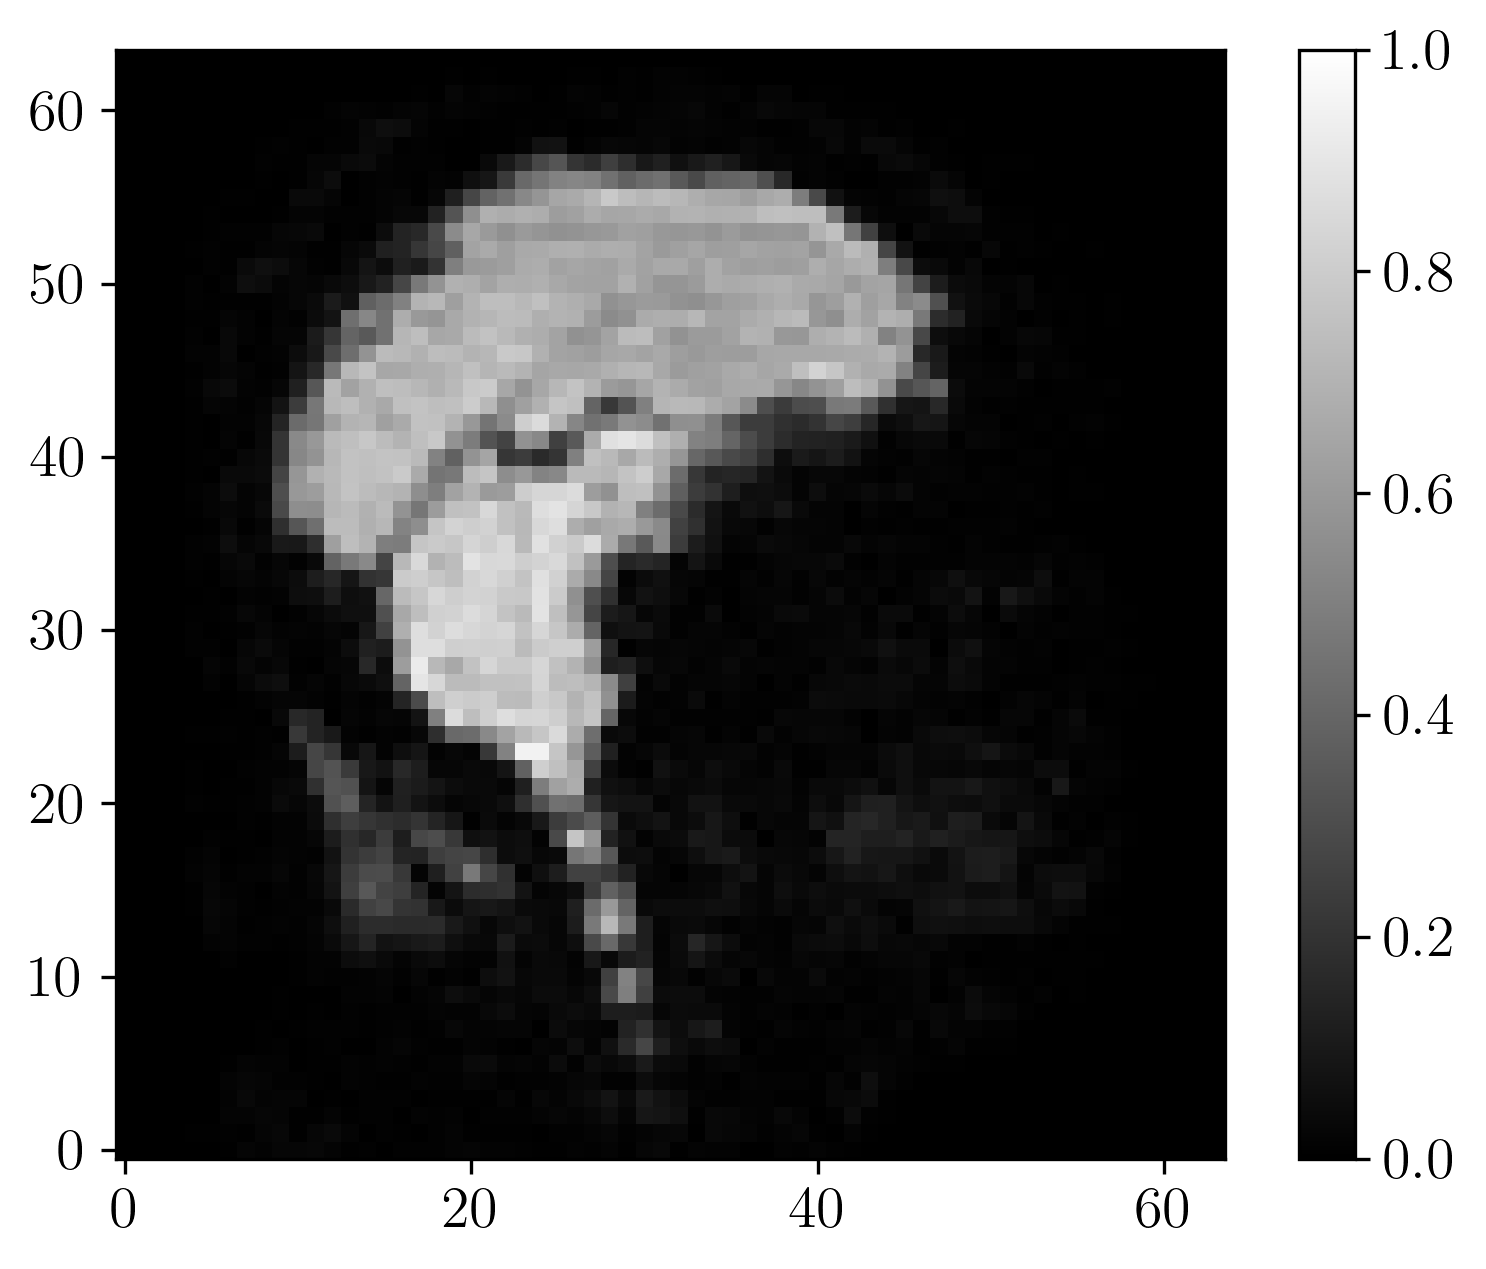
\includegraphics[width=0.33\textwidth]{sub-07-5-1-1000-37-20-_-_-predicted.png}}}
	\hfill
	\subfloat[Разность]{\label{fig:example-c}{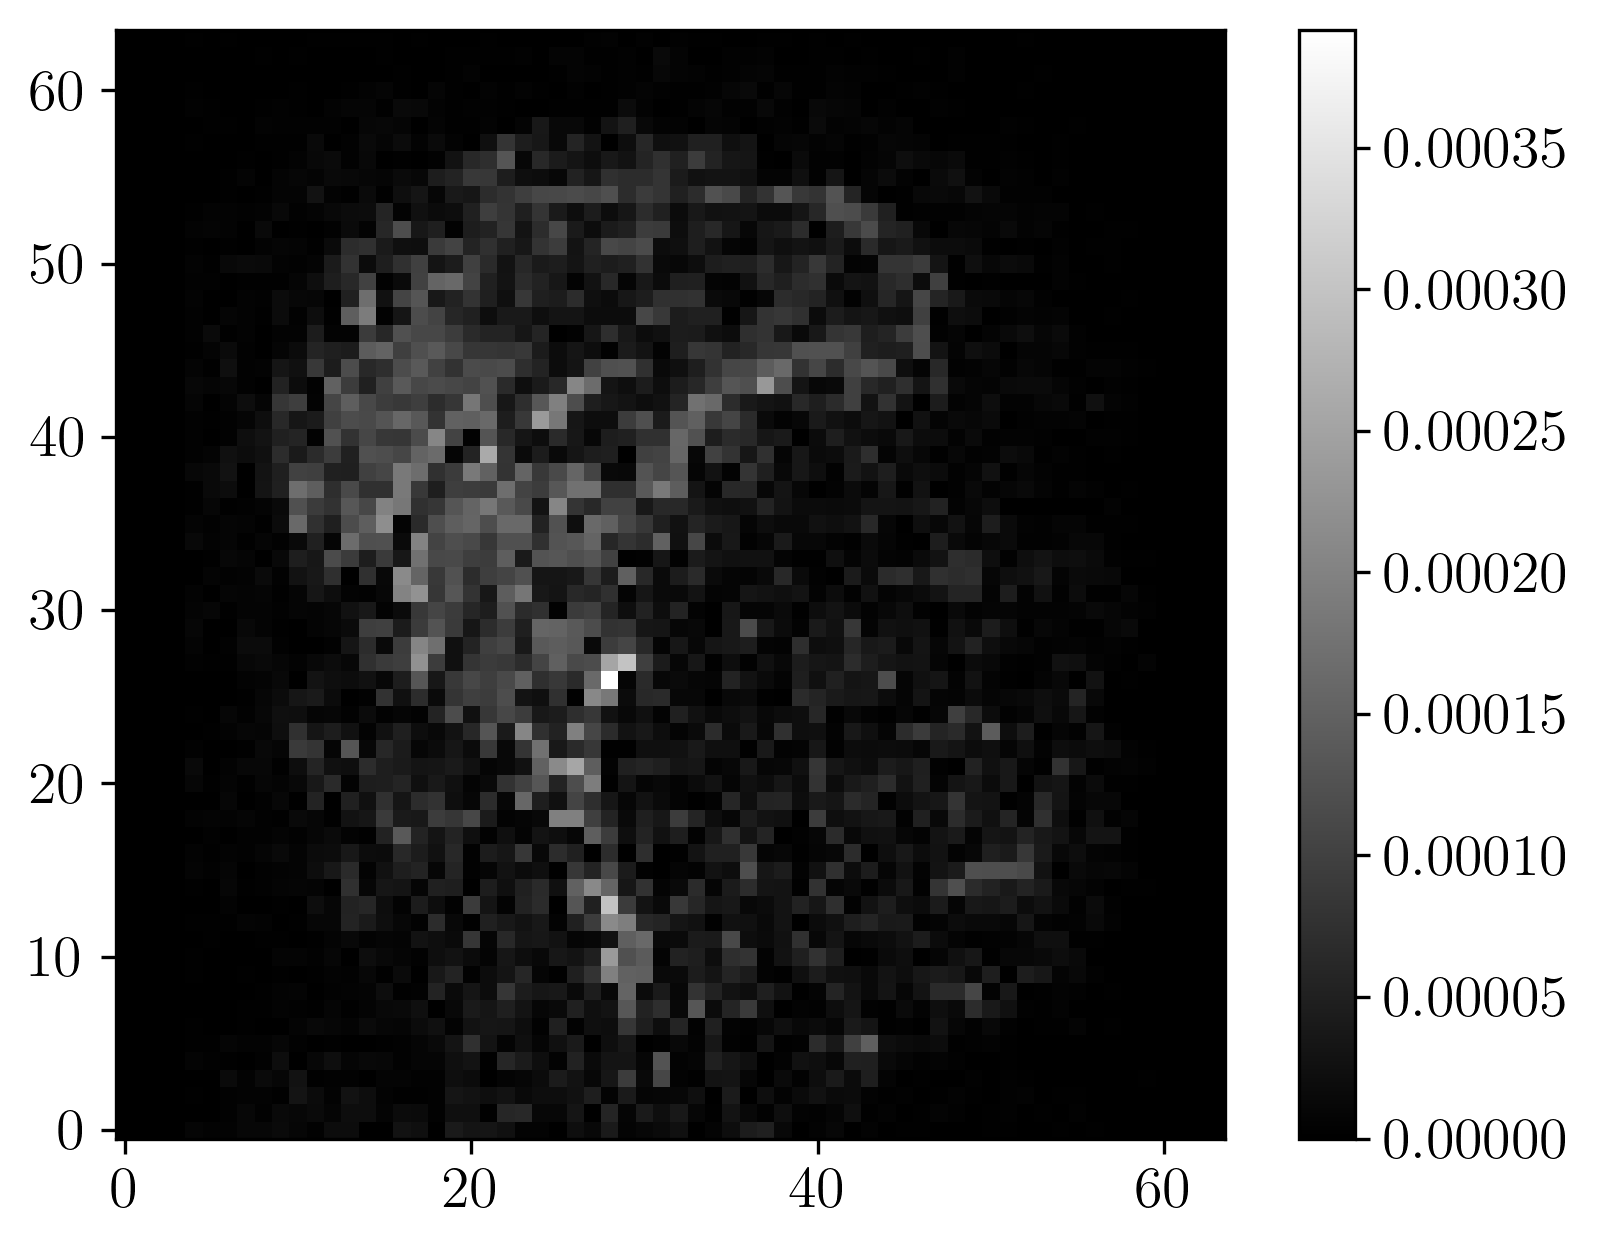
\includegraphics[width=0.33\textwidth]{sub-07-5-1-1000-37-20-_-_-difference.png}}}
	\caption{Срез снимка фМРТ из тестовой выборки}
	\label{fig:example}
\end{figure}

\paragraph*{Анализ времени задержки.}

Исследована зависимость качества восстановления от времени задержки.
Для примера был выбран 47-ой испытуемый.
На левом графике Рис.~\ref{fig:mse-dt} представлена зависимость метрики MSE
от времени задержки $\Delta t$.
Исследование \citep{anderson2006} подтверждает, что наиболее активная часть мозга
при рассматриваемом обследовании~--- затылочная доля.
Остальные части вносят шум в рассматриваемую зависимость.
В настоящей работе проведена локализация вышеупомянутой области, 
что видно на Рис.~\ref{fig:local}.
Для локализации области отсекаются нижняя треть и правые две трети объемного
томографического изображения.
Красным цветом выделена та зона, в которую попадают 3\% наиболее 
изменяющихся вокселей затылочной доли.
Для этого все воксели локализованной области были упорядочены по 
убыванию суммарного абсолютного изменения значений.
Далее были выбраны 3\% вокселей с наибольшими изменениями.
Произведен пересчет метрики MSE именно на этой части снимка.
Соответствующий график приведен справа на Рис.~\ref{fig:mse-dt}.

\begin{figure}[h!]
	\centering
	\subfloat[Истинный]{\label{fig:local-a}{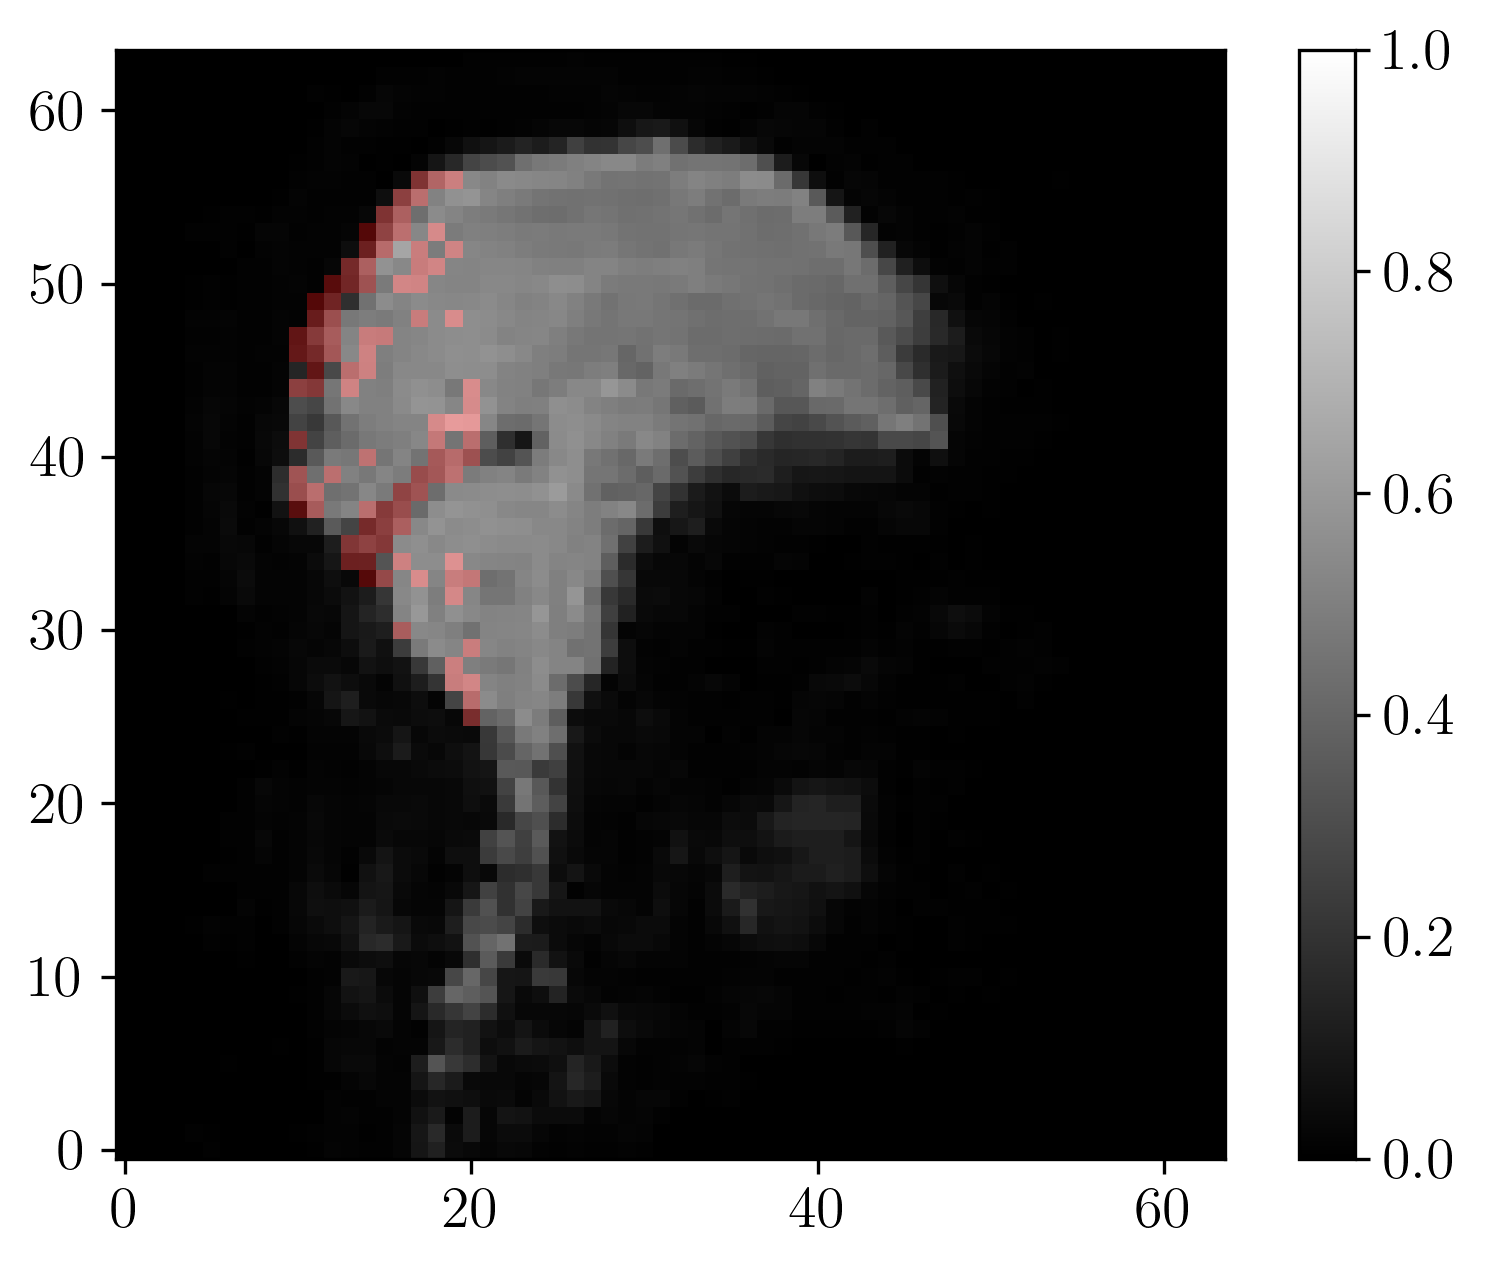
\includegraphics[width=0.33\textwidth]{local/sub-47-5-1-1000-37-20-_-_-test.png}}}
	\hfill
	\subfloat[Восстановленный]{\label{fig:local-b}{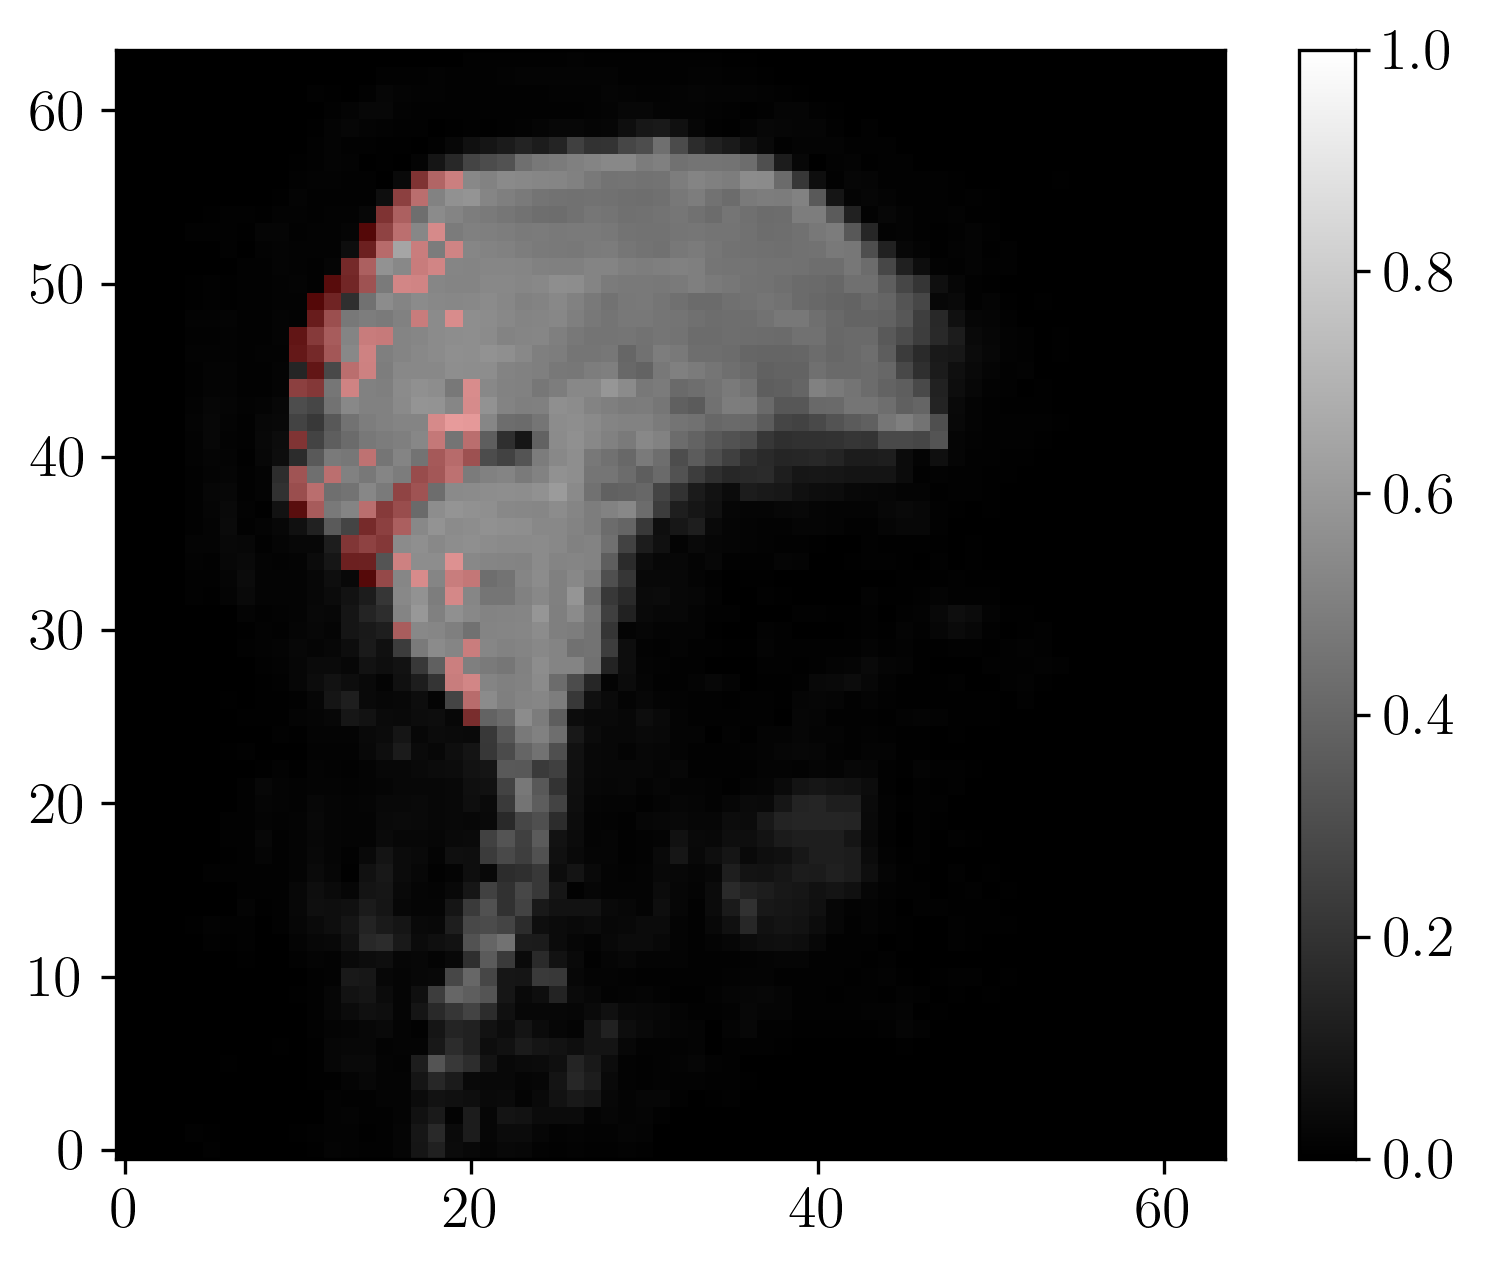
\includegraphics[width=0.33\textwidth]{local/sub-47-5-1-1000-37-20-_-_-predicted.png}}}
	\hfill
	\subfloat[Разность]{\label{fig:local-c}{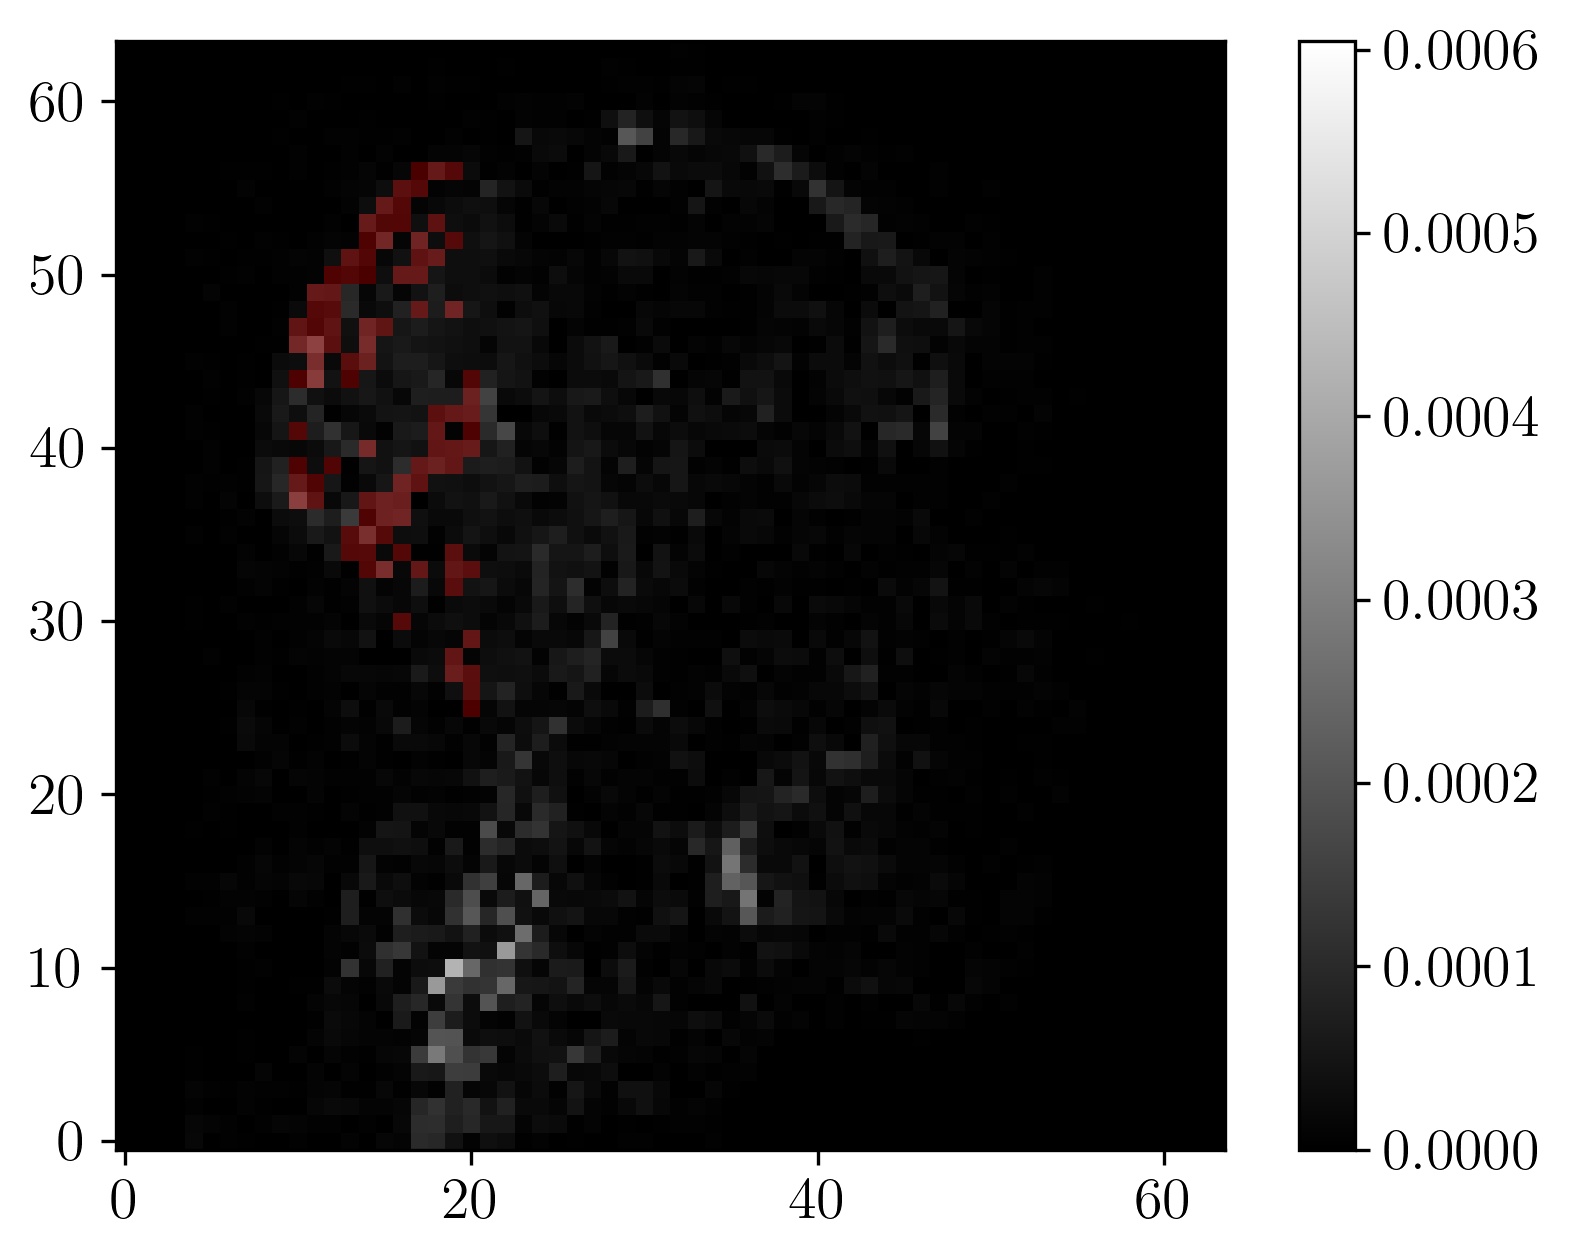
\includegraphics[width=0.33\textwidth]{local/sub-47-5-1-1000-37-20-_-_-difference.png}}}
	\caption{Локализация наиболее активной зоны}
	\label{fig:local}
\end{figure}

\begin{figure}[h!]
	\centering
	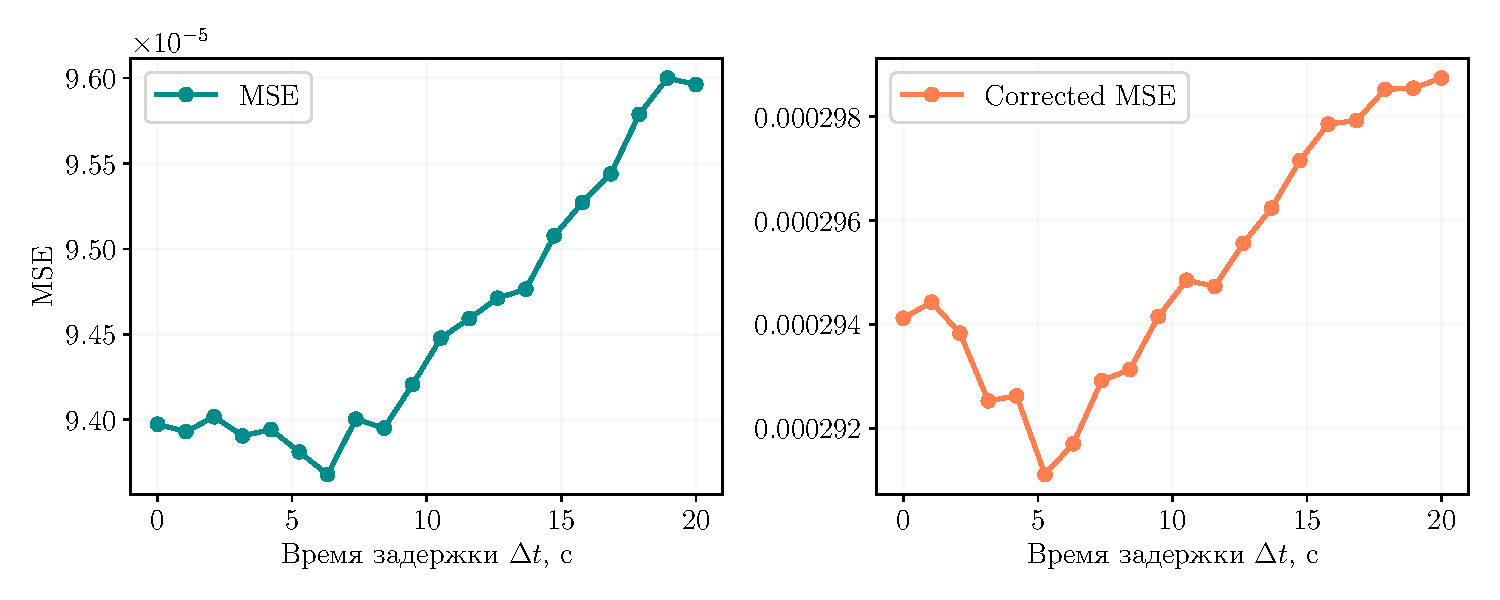
\includegraphics[width=\textwidth]{mse_dt.pdf}
	\caption{Зависимость метрики MSE от времени задержки}
	\label{fig:mse-dt}
\end{figure}

\paragraph*{Подбор оптимального коэффициента регуляризации.}

Проведен анализ зависимости MSE от коэффициента регуляризации $\alpha$.
Рассматривались коэффициенты сжатия 1, 2, 4 и 8.
Соответствующие графики приведены на Рис.~\ref{fig:mse-alpha}.
Для построения графика производилось усреднение по испытуемым.
Обозначены границы среднеквадратичного отклонения.
Из графиков видно, что оптимальное значение коэффициента $\alpha \approx 1000$.
Вид кривой сохраняется независимо от коэффициента сжатия снимков фМРТ.

\begin{figure}[h!]
	\centering
	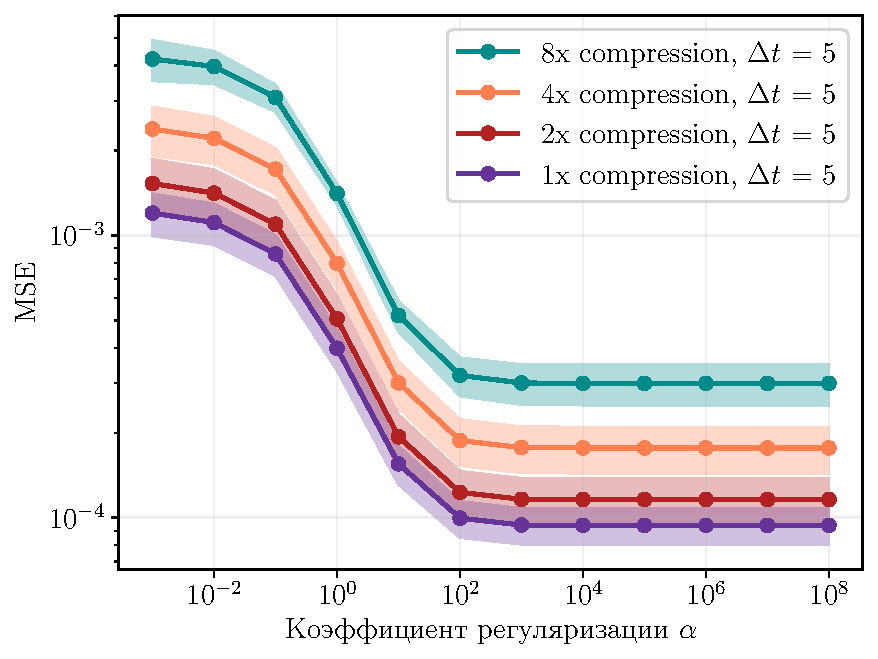
\includegraphics[width=0.65\textwidth]{subs_MSE_alpha.pdf}
	\caption{Зависимость метрики MSE от коэффициента регуляризации $\alpha$ на снимках из тестовой выборки}
	\label{fig:mse-alpha}
\end{figure}

\paragraph*{Влияние коэффициента сжатия снимков на время работы метода.}

Производится сравнение времени обучения модели при использовании различных
коэффициентов сжатия снимков фМРТ. Рассматриваются коэффициенты 1, 2, 4 и 8.
Для каждого значения коэффициента сжатия подсчитывается среднее по всем испытуемым
значение времени обучения модели. Вычисляется среднеквадратичное отклонение.
Результаты эксперимента приведены в Таблице~\ref{table:coeffs}.
Время работы метода существенно уменьшается при использовании
предварительного сжатия снимков фМРТ. 
Эксперимент с подбором оптимального коэффициента регуляризации
подтверждает то, что сжатие снимков не изменяет вид зависимостей.

\begin{table}[h!]
	\centering
	\caption{Зависимость времени обучения модели от коэффициента сжатия}
	\begin{tabular}{|c|c|c|}
		\hline
		Коэффициент сжатия & Среднее время, с & Среднеквадратичное отклонение, с \\ \hline \hline
		1 & 36.3 & 6.1 \\ \hline
		2 & 6.7 & 0.5 \\ \hline
		4 & 1.6 & 0.1 \\ \hline
		8 & 1.4 & 0.3 \\ \hline
	\end{tabular}
	\label{table:coeffs}
\end{table}

\paragraph*{Анализ распределения весов модели.}

Построен график распределения значений компонент вектора весов модели.
Для построения производилось усреднение по всем вокселям для 4-го испытуемого.
Результат представлен на Рис.~\ref{fig:w-distr}.
Веса модели не лежат в окрестности какого-то конкретного значения, 
то есть их распределение не вырождено.
Этот результат вполне согласуется с реальностью, поскольку человек во время просмотра
обращает внимание на определенные части кадра, например, персонажей или
другие детали.

\begin{figure}[h!]
	\centering
	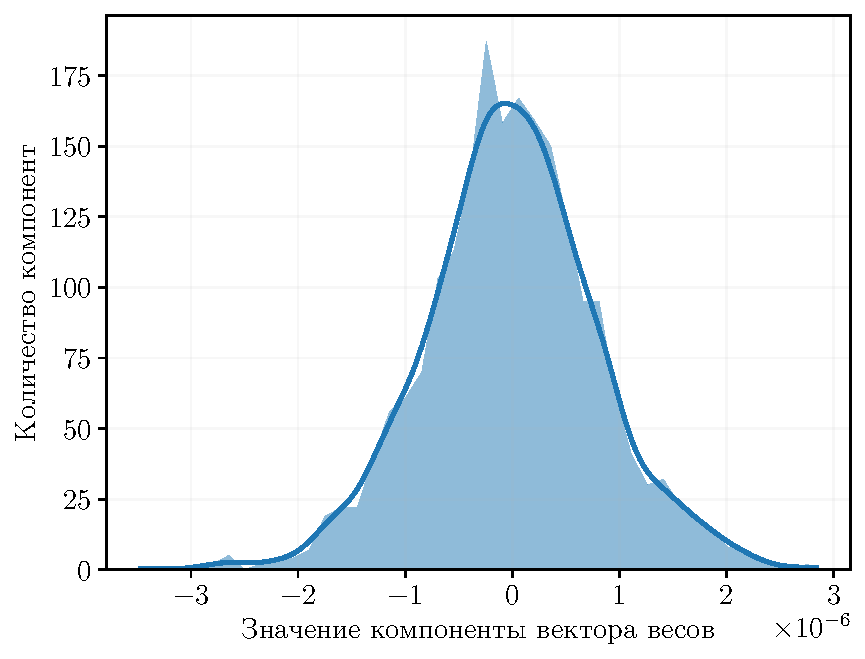
\includegraphics[width=0.65\textwidth]{distribution.pdf}
	\caption{Распределение значений компонент вектора весов}
	\label{fig:w-distr}
\end{figure}

\paragraph*{Гипотеза инвариантности весов модели относительно человека.}

Проведена проверка гипотезы инвариантности весов модели относительно человека:
использование матрицы весов одного испытуемого для восстановления снимков фМРТ другого.
Использовалась метрика MSE на тестовой выборке.
Результаты представлены в Таблице~\ref{table:inv}.
Рассмотрены 4-ый и 7-ый испытуемые. Матрица весов 4-го использовалась для восстановления
снимков 7-го.
Значения MSE практически совпадают. 

\begin{table}[h!]
	\centering
	\caption{Проверка гипотезы инвариантности весов модели относительно человека}
	\begin{tabular}{|c|c|c|c|}
		\hline
		Матрица весов & Истинная             & Подмешанная  & Разность        \\ \hline \hline
		MSE           & $9.7494 \cdot 10^{-5}$ & $9.7498 \cdot 10^{-5}$ & $3.96 \cdot 10^{-9}$ \\ \hline
	\end{tabular}
	\label{table:inv}
\end{table}

Аналогичный эксперимент проведен для каждой пары испытуемых.
Полученные результаты представлены на Рис.~\ref{fig:heatmap},
который был получен следующим образом.
Рассматривается некоторый испытуемый (соответствует строке матрицы), 
для него вычисляется MSE~--- <<истинный>>.
Далее рассматривается другой испытуемый (соответствует столбцу матрицы),
берется его матрица весов, и с помощью нее делается предсказание для первого 
испытуемого, затем вычисляется MSE~--- <<подмешанный>>. 
Разность между полученными MSE в процентах от <<истинного>> заносится в матрицу.
Положительное значение означает, что <<подмешанный>> MSE больше, чем <<истинный>>.
Отрицательное~--- что <<подмешанный>> меньше.
Идеальная модель должна приводить только к положительным значениям отклонений, однако,
как видно из Рис.~\ref{fig:heatmap}, в матрице есть и отрицательные значения.
Тем не менее, они достаточно малы, а именно соответствуют отклонениям порядка 1\%.
Это объясняется тем, что модель достаточно простая, а потому обладает
высокой обобщающей способностью.
Однако это не мешает сделать вывод о том, что данные не противоречат гипотезе 
об инвариантности весов модели относительно человека.

\begin{figure}[h!]
	\centering
	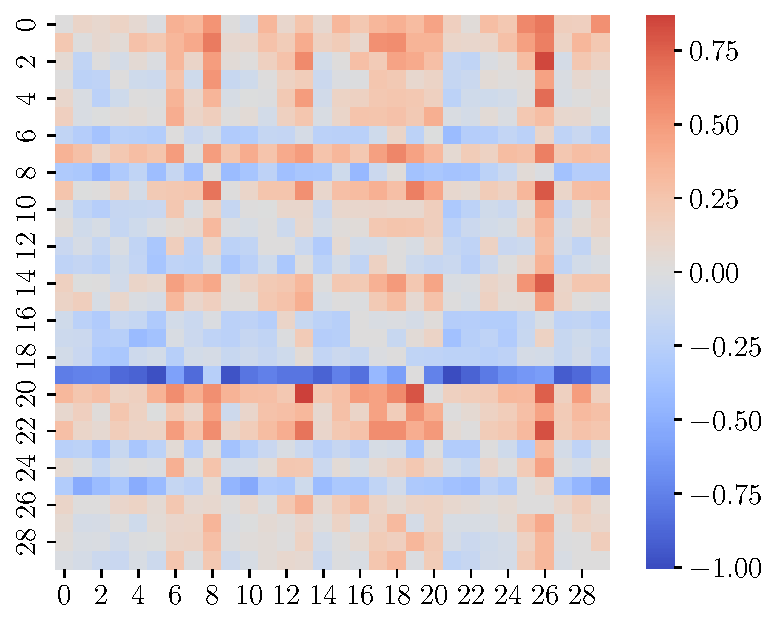
\includegraphics[width=0.5\textwidth]{heatmap.pdf}
	\caption{Изменение MSE при предсказании на подмешанной матрице весов (в процентах)}
	\label{fig:heatmap}
\end{figure}

\paragraph*{Корректность метода.}

Рассмотрено качество работы метода на неинформативных данных.
В качестве матрицы объекты-признаки $\bX$ взята матрица, целиком состоящая из единиц.
Произведено сравнение с результатами на настоящей матрице признакового описания.
К первому снимку 35-го испытуемого последовательно прибавляются все восстановленные
изменения значений вокселей.
В результате имеем последний снимок последовательности. На Рис.~\ref*{fig:recover}
представлены срезы последнего истинного и восстановленного снимков из тестовой выборки.
На Рис.\myfigref{fig:recover}{fig:recover-c} видна разность между ними.
Результаты на неинформативных продемонстрированы на Рис.~\ref*{fig:random}.
Разность между истинным и восстановленным снимками при работе с неинформативными данными
значительно выше, что подтверждает наличие зависимости между показаниями датчиков и
изображениями из видеоряда. Численные результаты приведены в Таблице~\ref{table:random}.

\begin{figure}[h!]
	\centering
	\subfloat[Истинный]{\label{fig:recover-a}{\includegraphics[width=0.33\textwidth]{original/sub-35-5-1-1000--1-20-_-_-recovered-test.png}}}
	\hfill
	\subfloat[Восстановленный]{\label{fig:recover-b}{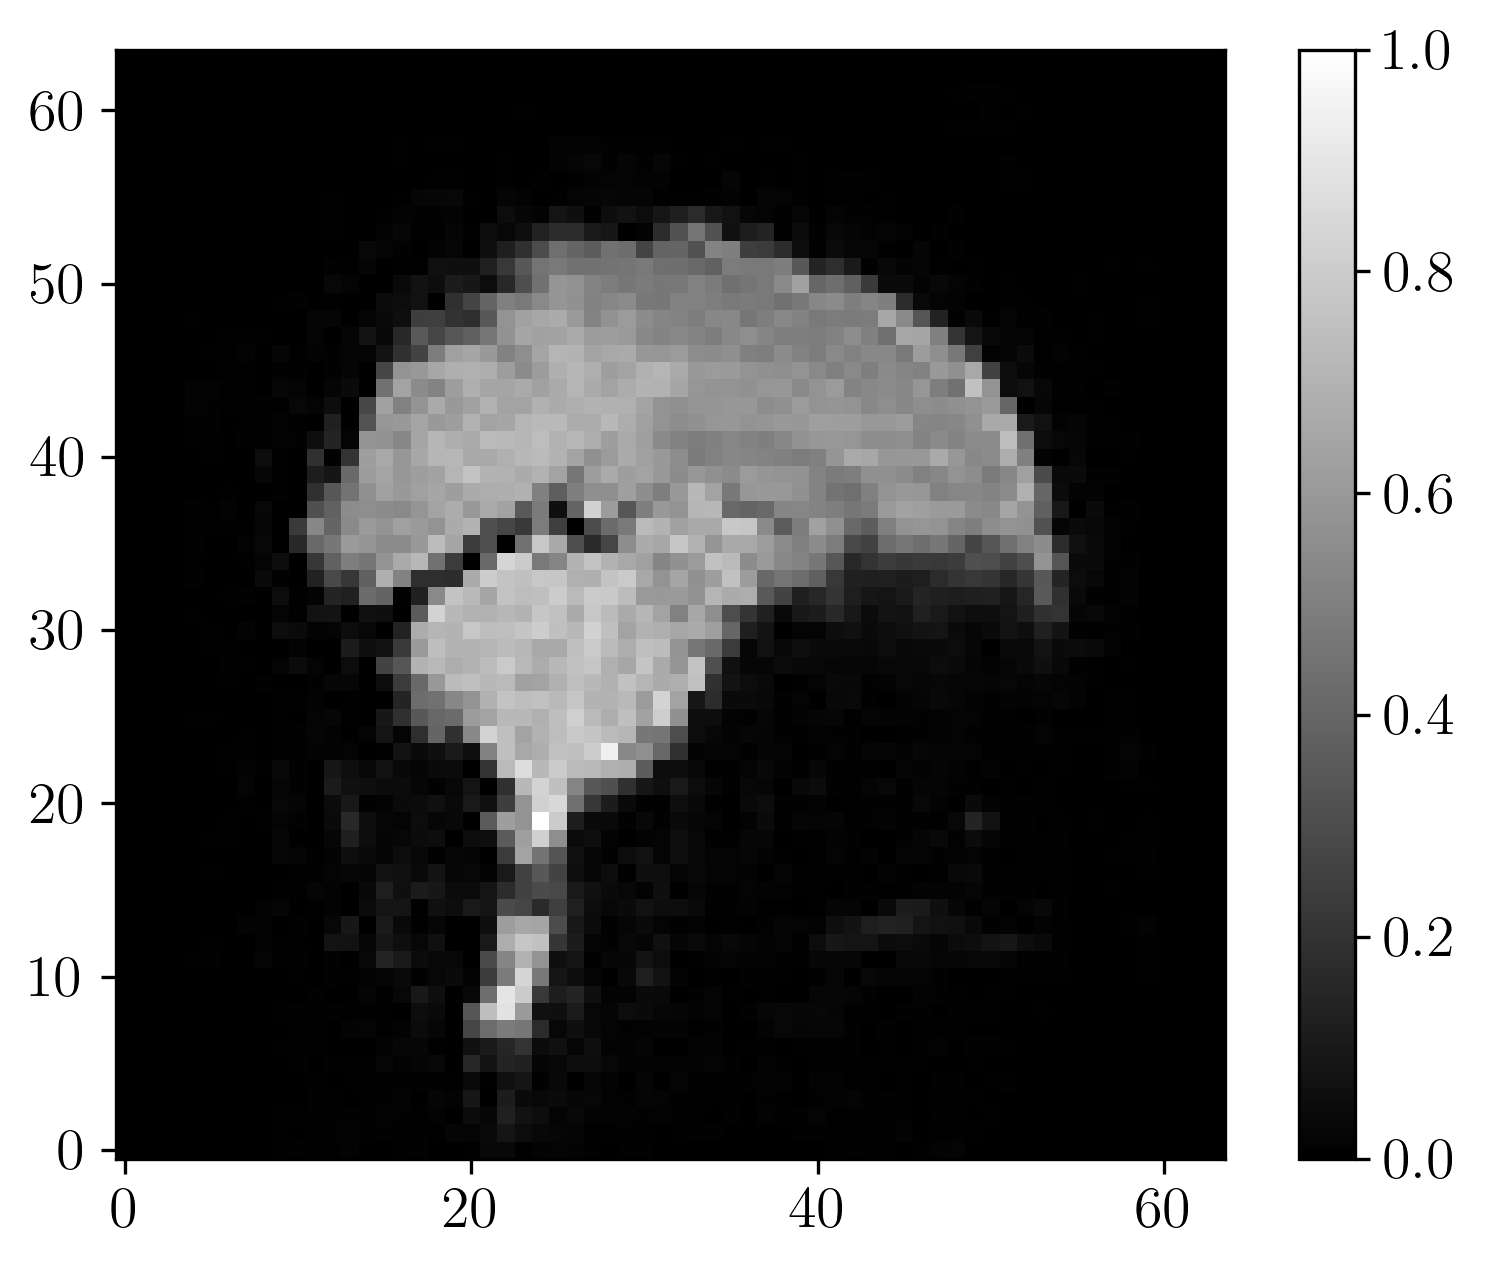
\includegraphics[width=0.33\textwidth]{original/sub-35-5-1-1000--1-20-_-_-recovered-predicted.png}}}
	\hfill
	\subfloat[Разность]{\label{fig:recover-c}{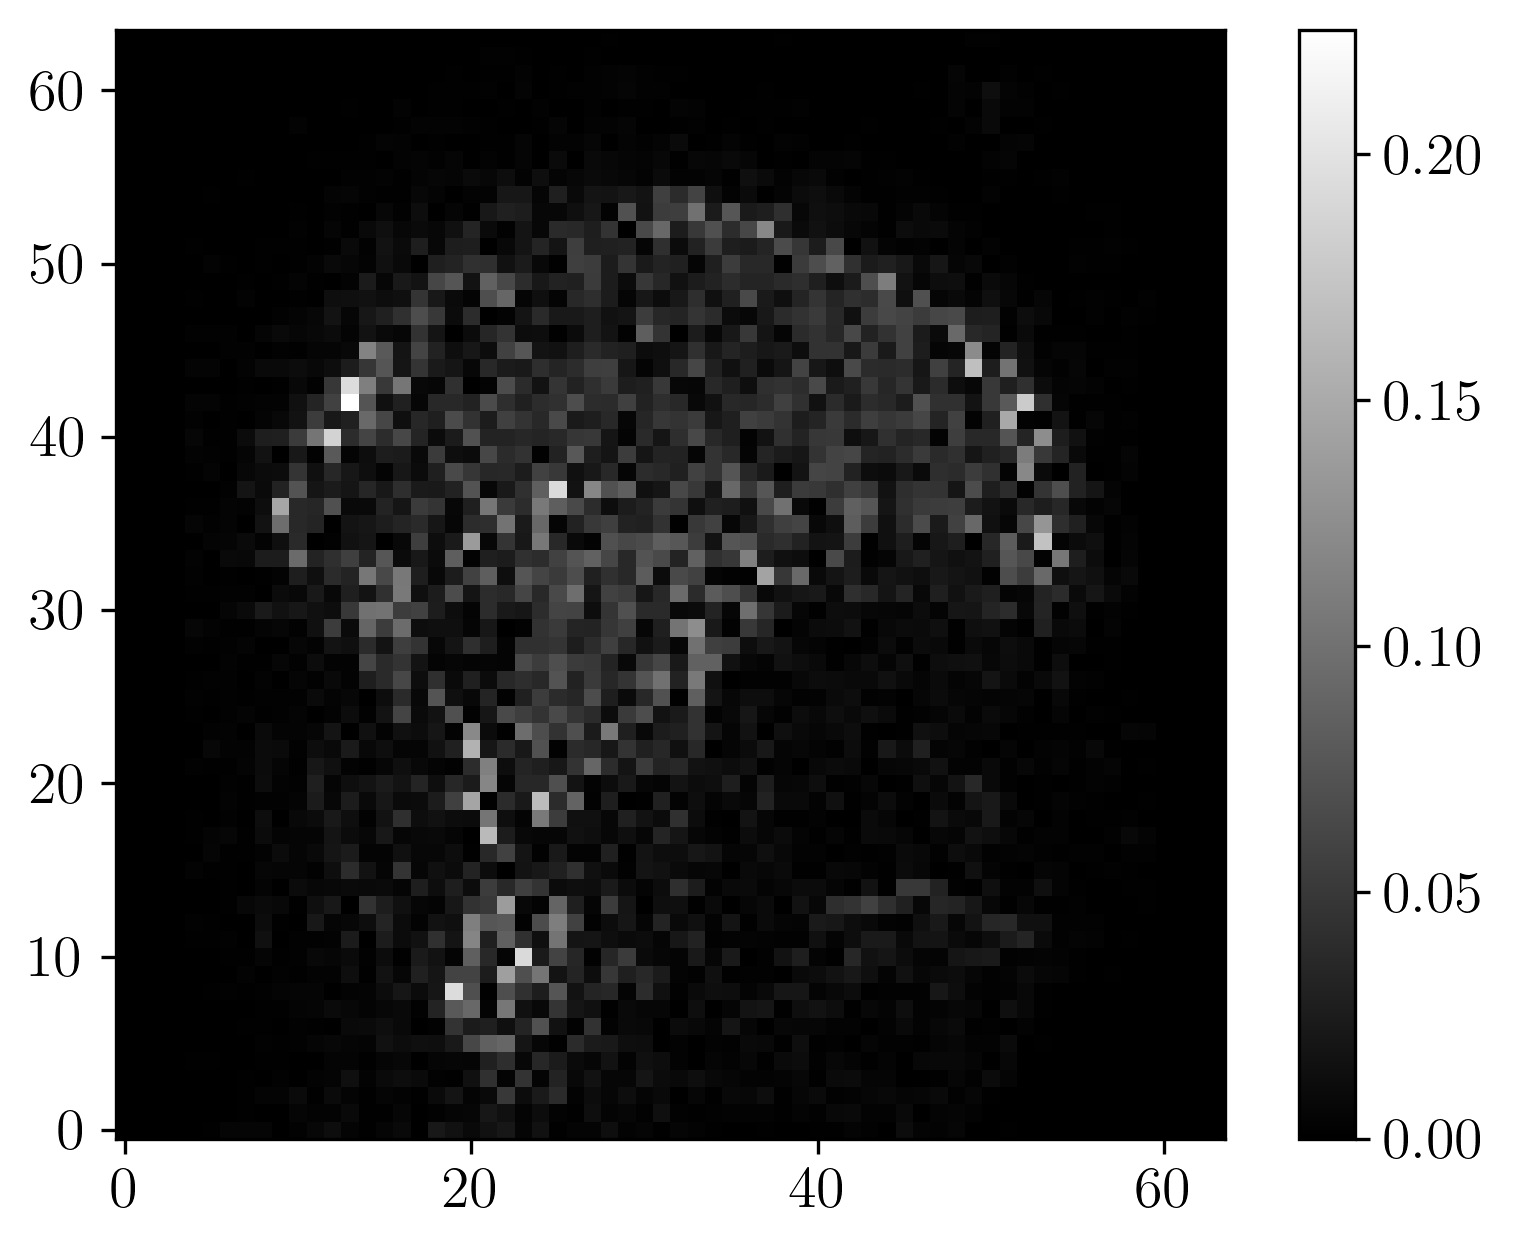
\includegraphics[width=0.33\textwidth]{original/sub-35-5-1-1000--1-20-_-_-recovered-difference.png}}}
	\caption{Срез снимка фМРТ из тестовой выборки}
	\label{fig:recover}
\end{figure}

\begin{figure}[h!]
	\centering
	\subfloat[Истинный]{\label{fig:random-a}{\includegraphics[width=0.33\textwidth]{noised/sub-35-5-1-1000--1-20-_-_-recovered-test.png}}}
	\hfill
	\subfloat[Восстановленный]{\label{fig:random-b}{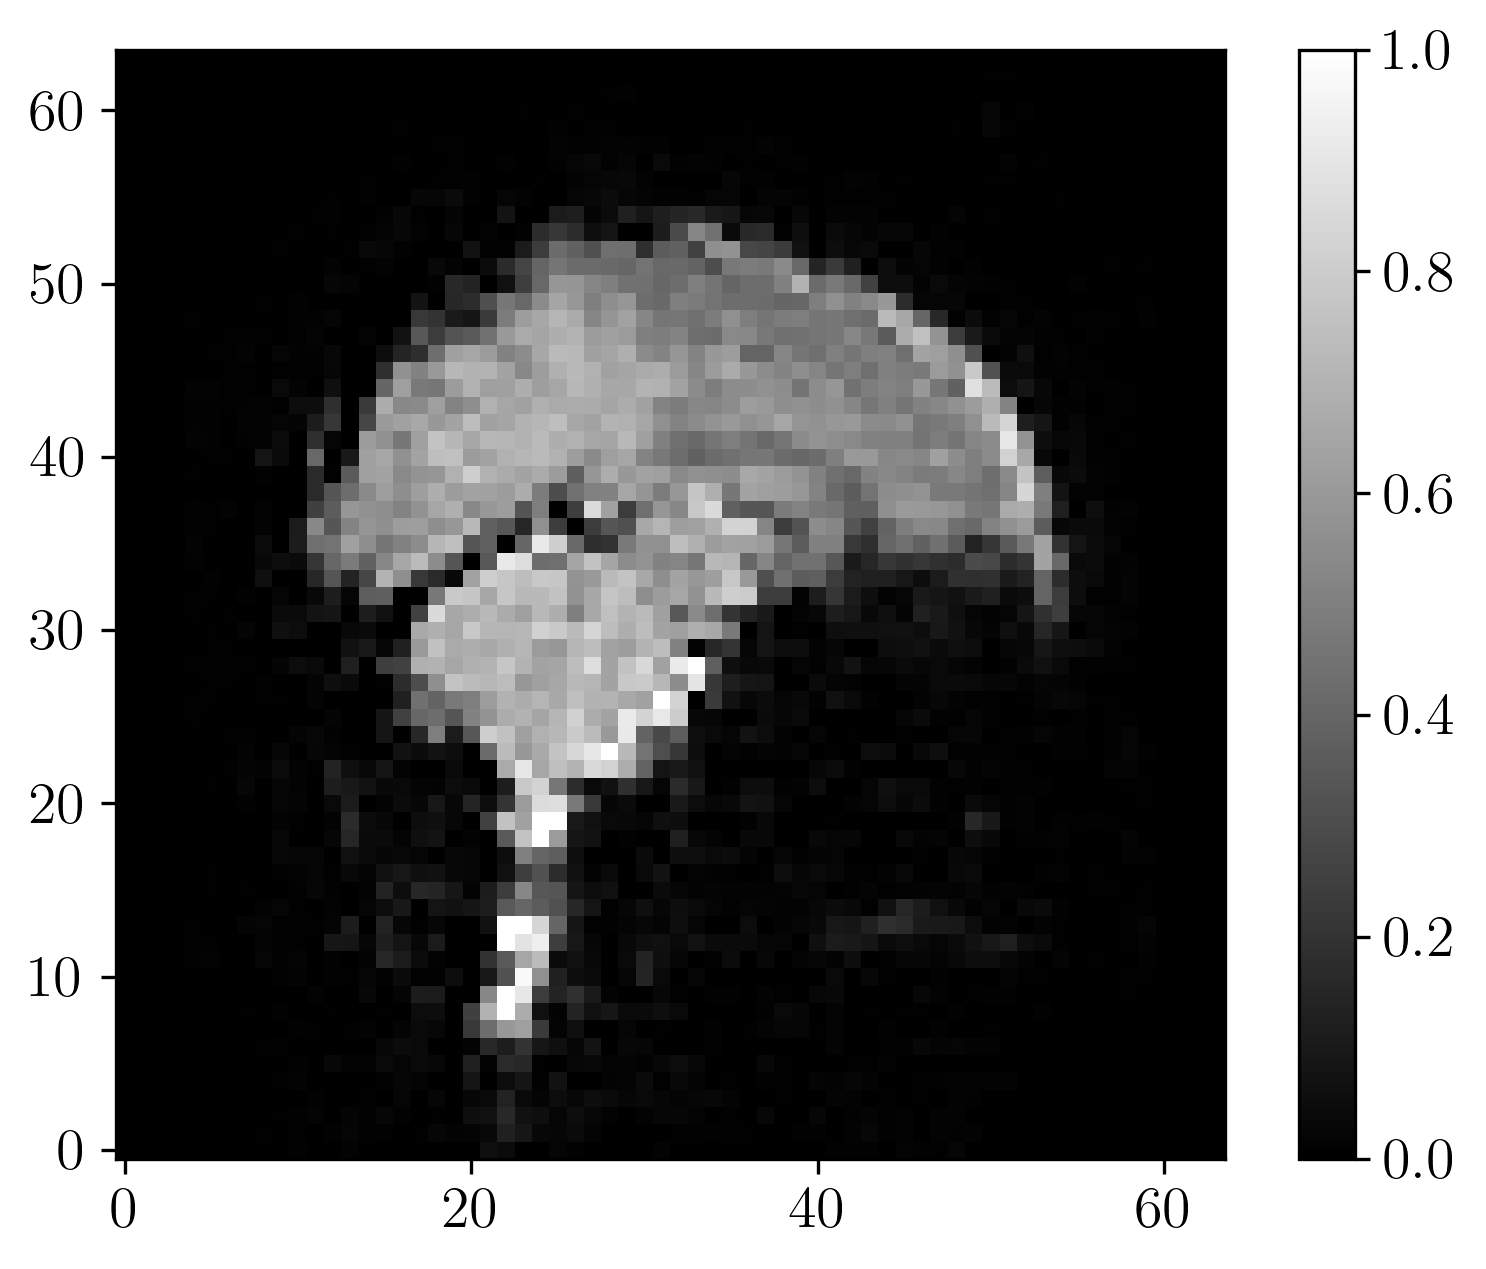
\includegraphics[width=0.33\textwidth]{noised/sub-35-5-1-1000--1-20-_-_-recovered-predicted.png}}}
	\hfill
	\subfloat[Разность]{\label{fig:random-c}{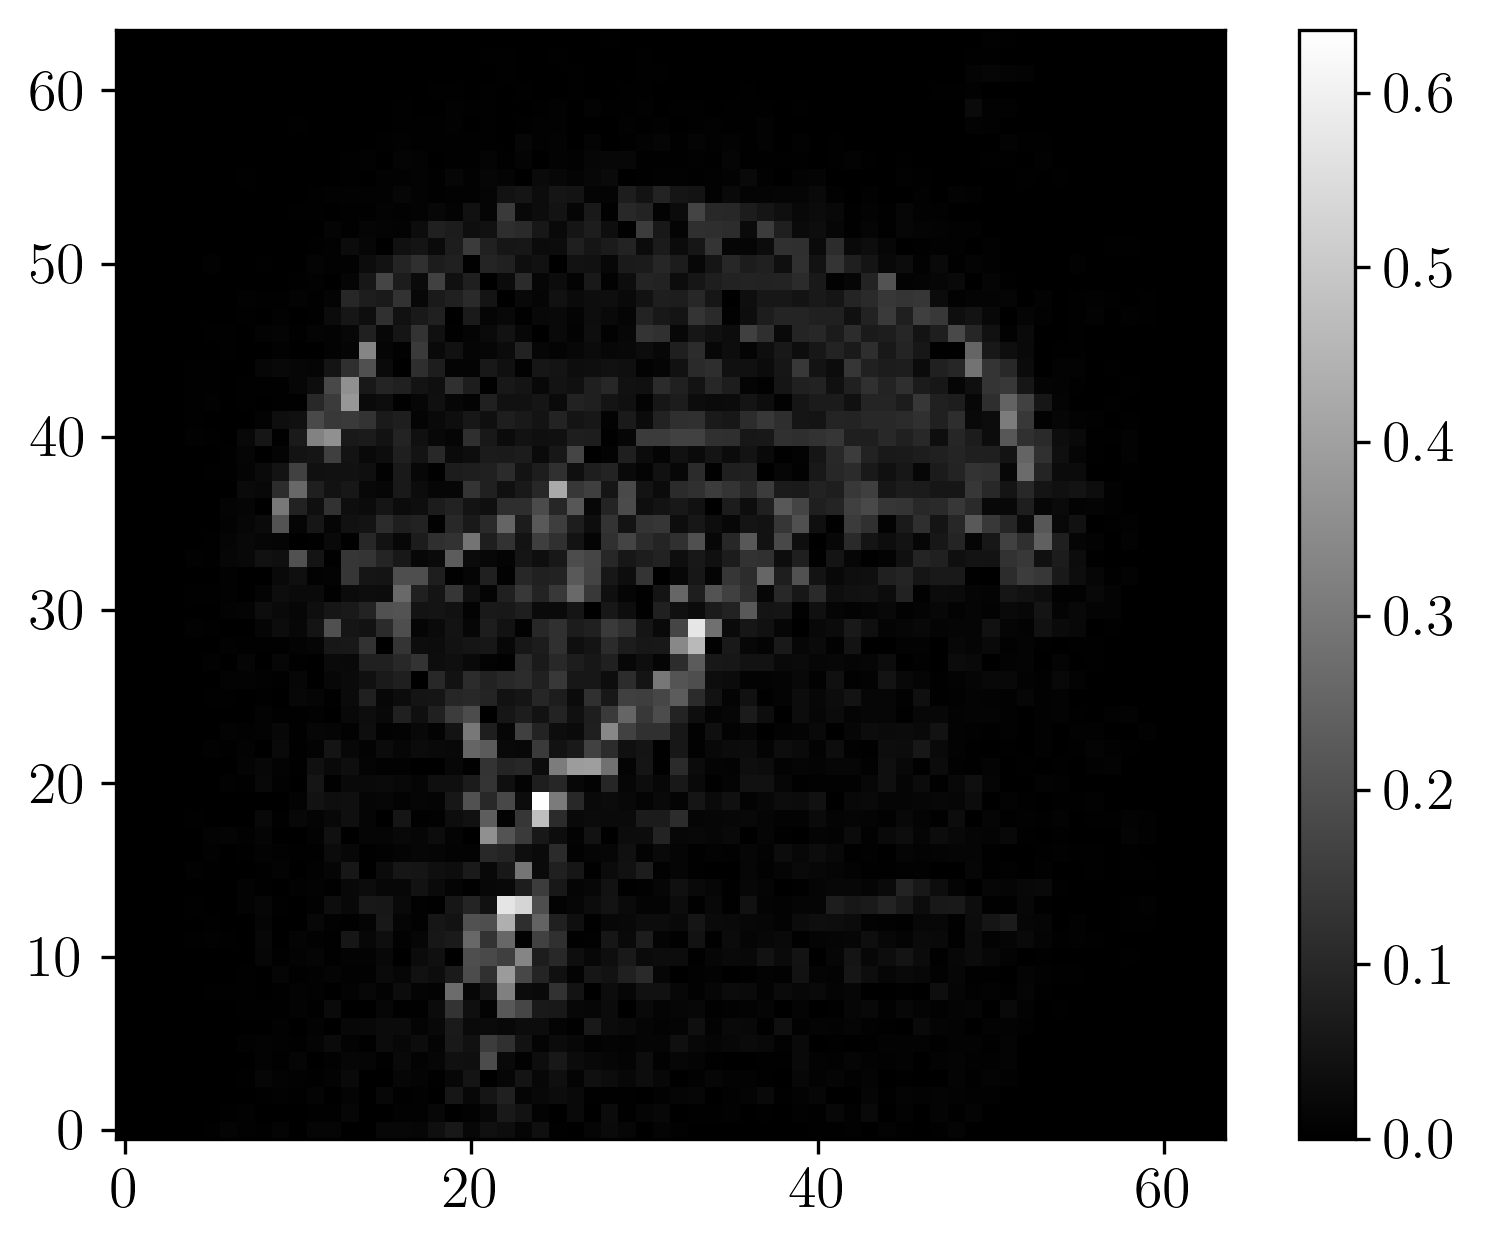
\includegraphics[width=0.33\textwidth]{noised/sub-35-5-1-1000--1-20-_-_-recovered-difference.png}}}
	\caption{Срез снимка фМРТ из тестовой выборки (на неинформативных данных)}
	\label{fig:random}
\end{figure}

\begin{table}[h!]
	\centering
	\caption{Качество работы метода на неинформативных данных}
	\begin{tabular}{|c|c|c|c|}
		\hline
		Выборка & Истинная          & Неинформативные данные & Разность \\ \hline \hline
		MSE     & $4.87 \cdot 10^{-4}$ & $1.76 \cdot 10^{-3}$ & $1.27 \cdot 10^{-3}$ \\ \hline
	\end{tabular}
	\label{table:random}
\end{table}


\paragraph*{Корреляционный анализ данных.}

Проведем дополнительное исследование данных, представленных в выборке \citep{Berezutskaya2022}.
Как было сказано ранее, в датасете также есть информация о времени появления
и исчезновения отдельных объектов в кадре. Используем эту информацию, чтобы составить признаковое
описание изображений видеоряда меньшей размерности. Всего есть информация о 135 различных объектах.
Закодируем каждое изображение вектором из 0 и 1 размерности 135, где 0 соответствует отсутствию
объекта в кадре, а 1~--- его наличию.

Объект, который чаще всего появляется и пропадает из кадра~--- Пеппи, главная героиня фильма,
фрагмент которого показывался испытуемым. Число различных фрагментов, где она находится в кадре,
равно 26. Исследуем кросс-корреляцию временного ряда, соответствующего этому объекту, с 
временным рядом снимков фМРТ.

\begin{figure}[h!]
	\centering
	\subfloat[Истинный]{\label{fig:occur-a}{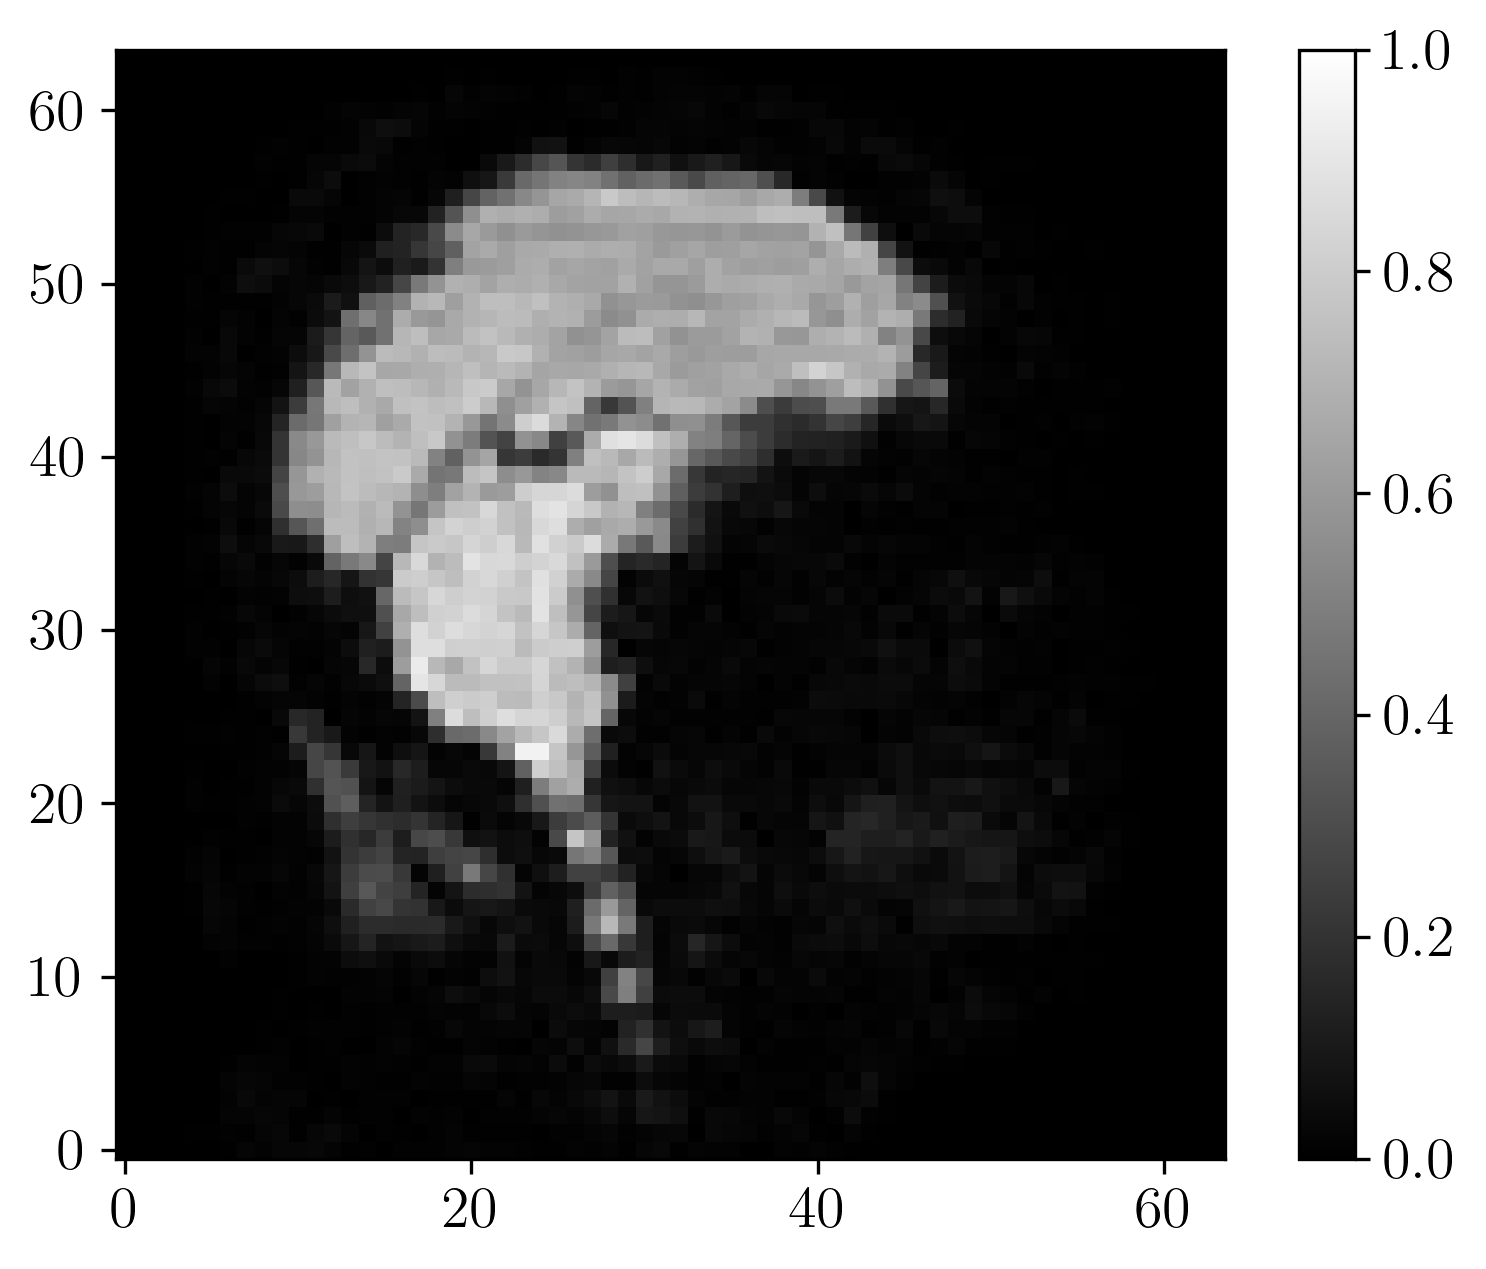
\includegraphics[width=0.33\textwidth]{scan_test.png}}}
	\hfill
	\subfloat[По кросс-корреляции]{\label{fig:occur-b}{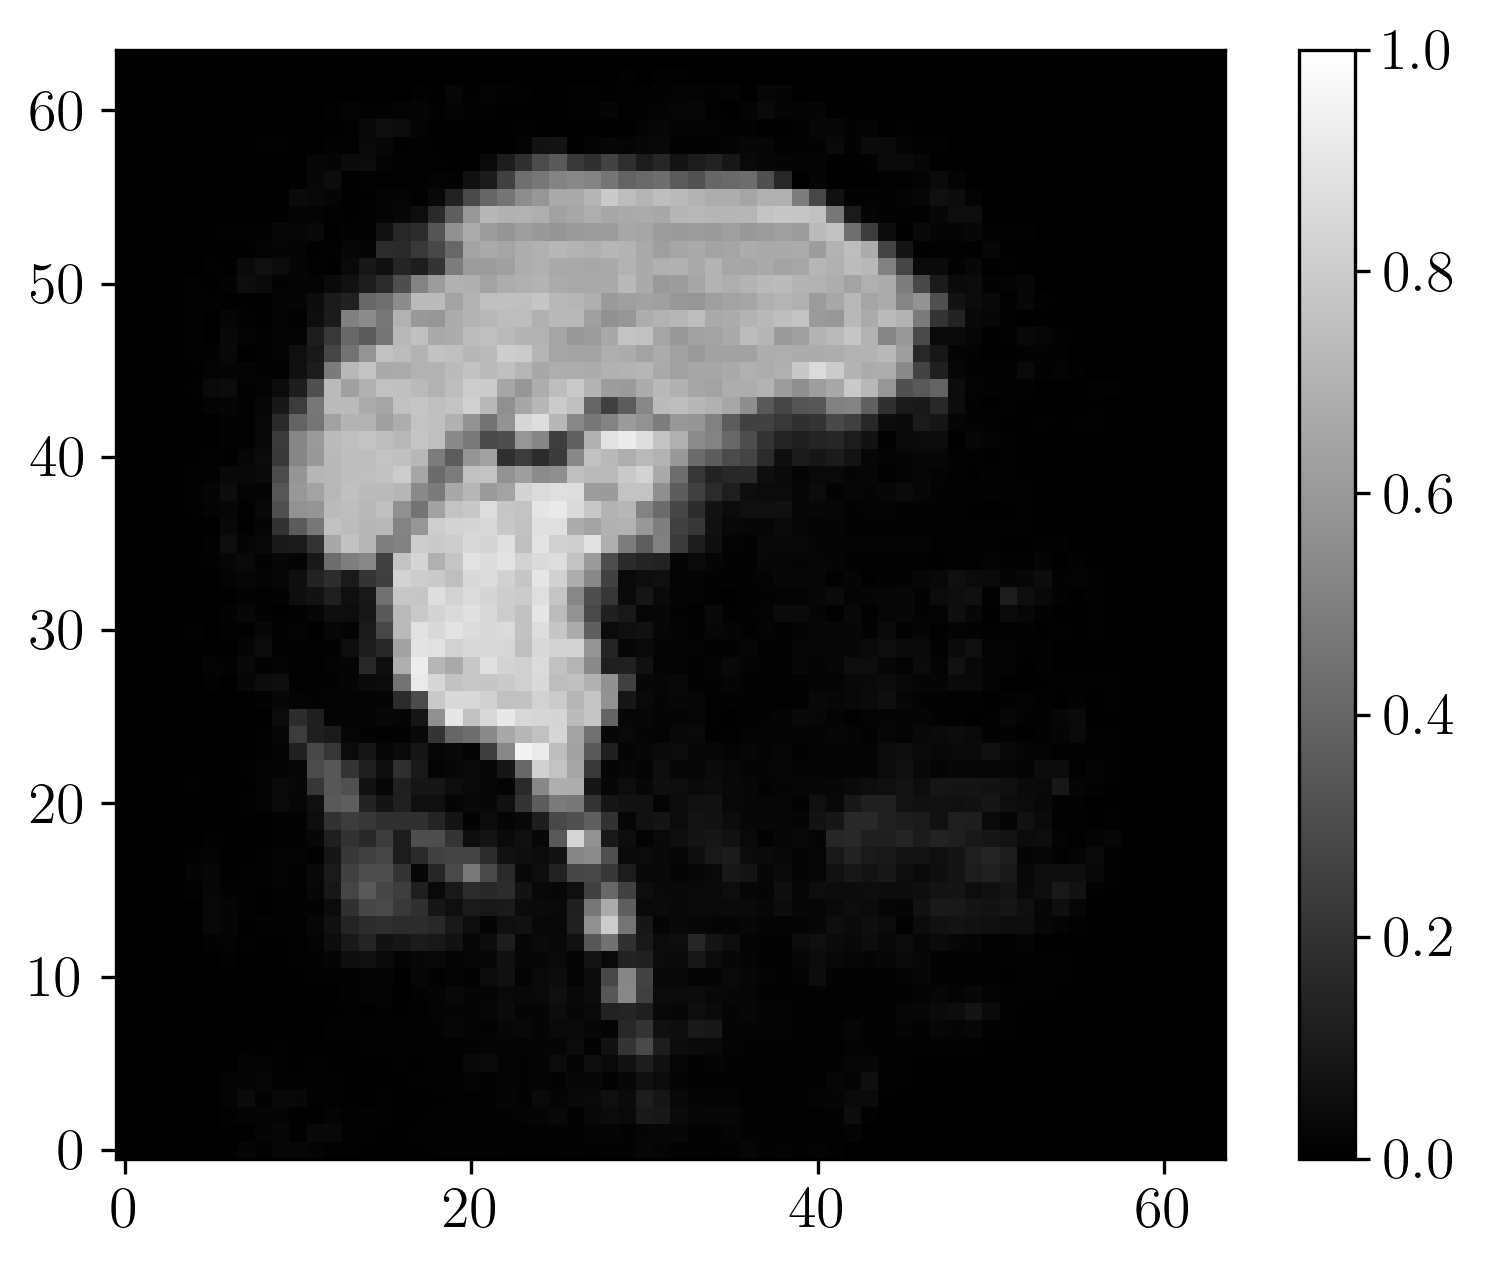
\includegraphics[width=0.33\textwidth]{scan_cross_correlation.png}}}
	\hfill
	\subfloat[Разность]{\label{fig:occur-c}{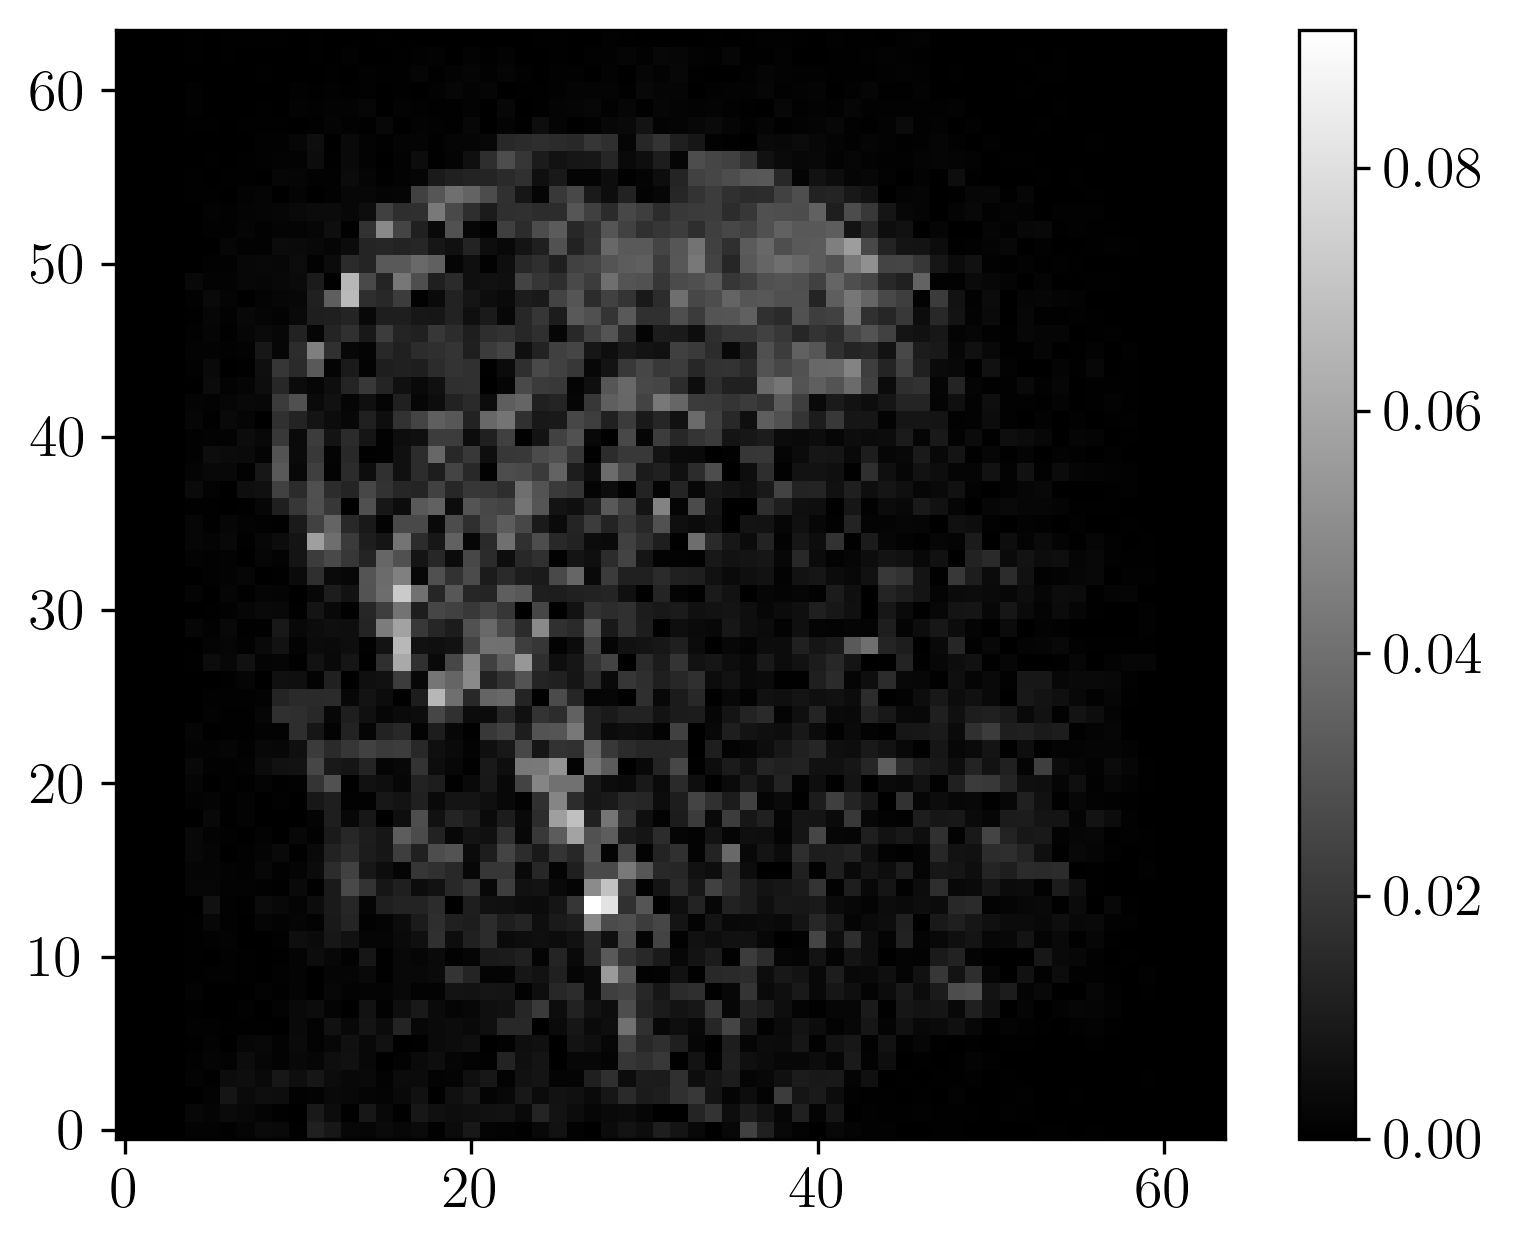
\includegraphics[width=0.33\textwidth]{scan_difference.png}}}
	\caption{Срез снимка фМРТ из тестовой выборки (в сравнении с кросс-корреляционным)}
	\label{fig:occur}
\end{figure}

На Рис.~\myfigref{fig:occur}{fig:occur-a} представлен настоящий снимок фМРТ из тестовой выборки. В качестве примера был выбран
7-ой испытуемый, 20-ый срез по первой координате 37-го снимка в последовательности.
На Рис.\myfigref{fig:occur}{fig:occur-b} представлен снимок, который был получен по значениям кросс-корреляционной функции.
А именно, для каждого вокселя был получен временной ряд, соответствующий его изменению во времени.
Далее была подсчитана его кросс-корреляционная функция с выбранным объектом.
Затем было выбрано смещение, которое соотвествует времени задержки порядка 5 секунд.
Полученное число для каждого вокселя было отнормировано на отрезок $[0; 1]$.

Как видно из Рис.\myfigref{fig:occur}{fig:occur-c}, снимки практически совпадают. 
Среднеквадратичное значение ошибки MSE равно $7.8 \cdot 10^{-5}$.
Это еще раз подтверждает факт того, что мозг человека реагирует 
на появление и исчезновение конкретных объектов из кадра.

\newpage

\section{Заключение}

В работе рассматривается задача восстановления зависимости между показаниями
датчиков фМРТ и восприятием внешнего мира человеком.
Предлагается метод аппроксимации последовательности снимков фМРТ по видеоряду. 
Метод учитывает время гемодинамической ответной реакции~--- время задержки между изображениями из видеоряда и снимками фМРТ. 
Для каждого вокселя снимка фМРТ независимо строится линейная модель. 
Каждая линейная модель строится в предположении марковости последовательности снимков фМРТ. 
В ходе экспериментов для каждого испытуемого подбирается оптимальное значение времени задержки. 
Оптимальное значение находится из анализа графика зависимости MSE от времени задержи.
Подбирается коэффициент регуляризации. 
Исследуется влияние коэффициента сжатия снимков фМРТ на время обучения модели.
Предполагается, что за информацию со зрительных органов отвечает затылочная доля мозга.
Производится поправка MSE на основе локализации этой области и выбора наиболее изменяющихся вокселей. 
При таком построении график имеет характерный минимум, отвечающий оптимальному значению времени задержки.
Полученное значение времени задержки согласуется с нейробиологическими сведениями.
Экспериментальные значения MSE малы, что говорит о наличии корреляции между данными. 
Учитывается изменение изображений в видеоряде, так как распределение весов модели не вырождено.
Проверена гипотеза инвариантности весов модели относительно человека. 
Корректность метода подтверждается экспериментами со случайными данными.

\newpage

\bibliographystyle{unsrt}
\bibliography{fMRI_2023.bib}

\end{document}